\newcommand{\comment}[1]{}

\comment{

%—————————————————————————————————————————————————————————————————%

[Jamie's Layout]

1. Intro 
  1.n-1. Significance, future work, applications. 
  1.n Organization of paper. 
2. Box framework (Keep? You two decide.)  
3. GHZ stuff you guys did. 
4. SDP continuity I did. 
5. Cheating in P
  5.1. Cheating Alice in P, perfect case. (Include the numerics.)
  5.2. Cheating Alice in P, imperfect case. (Discuss continuity.) [This is short.]
  5.3. Cheating Bob in P, perfect case. (Include the numerics.)
  5.4. Cheating Bob in P, imperfect case. (Discuss continuity.) [This is short.]
6. Cheating in Q
  6.1 Cheat vectors for Bob in Q. (Discuss continuity.) 
  6.2. Final composition details. (Include the numerics.) [This is short.] 
7. Conclusions. 
8. Computational platform, acknowledgements, and references. 


%—————————————————————————————————————————————————————————————————%

[Atul (after discussing with Tom)]

Here's what I propose based on my discussion with Tom.

Rationale: It appears that Jamie's idea is to have a long rather detailed introduction and then have all the details appear in the order of logical necessity for the final result. 

I have two issue: 

Issue 1:
While I like the idea, I think it is neither long enough to be fully clear (which means it causes redundancy later), nor short enough to be a quick preview of what's to come. But I feel its easy to fix—we remove the explicit protocols because we anyway don't use their details; our ideas are quite general. This would let us state the protocols clearly in one place (and exactly once), avoiding redundancy without any significant loss to the introduction's quality.

Issue 2:
I think it is worthwhile splitting the analysis into asymptotic analysis and finite n analysis. This is because if I, as a reader, get interested in the article then after reading the introduction, I want to be able to see concretely how something close to the final statement can be proved first, if it is easier. The details about finite size effects I may even decide to skip until I actually need it somewhere. Conversely, I may be only interested in seeing how finite sized effects are handled and then too it helps to have them separated. (Been there!)
I think one way of achieving such a structure is to introduce the protocols formally (see below) in a separate section, and state their security guarantees. Then formally introduce the compositions (with the relevant notation), make the final result appear plaussible and state it. With these in place, give the asymptotic proof for the assertions and then fill in the remaining steps for the full proof.

General remark:
Tom: Earlier, since we were not sure about Bob self-testing, I had changed the protocol I use for illustrating abort phobic compositions—I started using P. We can now directly use Q but this would mean you'll have to modify the figure. Sorry about that.

1. Introduction 
	n-1. Significance, future work, applications. 
	n. Organisation of the article 

	[remarks]
	* Essentially unchanged except that the explicit protocols I and P are only referenced; they appear later
	* The details about intermediate steps appear only as a floating table later and are only referenced in the introduction; the notation for composition only appears there with some explanation in the caption
	* Cheat vectors are defined properly here.
2. Protocols (First technique)
	[remark] This is where all the protocols 
	a. Original with formal security statement
		[remark: This will contain an informal description of how boxes can be transmitted over quantum channels; the details go in the appendix]
	b. Alice self tests with security statement
	c. Bob self tests with security statement
		[remark: Since cheat vectors are already defined and motivated, I would mention that they can be optimized over as SDPs]
3. Compositions (Second technique)
	a. Standard
		[remark: I wouldn't remove these because it really helps seeing what is happening]
	b. Abort phobic
4. Security proof | Asymptotic	
	a. Asymptotic self-testing
		Explain the asymptotic setting clearly; going from ⟨Test_GHZ⟩=1 to GHZ state and measurement up to local isometries.
	b. Alice self tests
	c. Bob self tests
5. Security proof | Finite n
	State in words the lemmas (and reference them) we use to prove the continuity statement. Then state and prove the continuity result.
	a. Robust self testing
	b. Estimating GHZ
	c. SDP continuity
6. Acknowledgements, Computational platform (+ link to the code)
7. Conclusion [QUESTION: is this really needed?]

A. The Box framework


%—————————————————————————————————————————————————————————————————%
[Tom's List]
To be practical (I’m really surprising myself here), we should make a small todo list and give each one some task that they complete by some deadline. I’m suggesting the following distribution of tasks

Content:

Jamie: Fill in the details of the continuity proof (continuity under changes of the constraints, currently there is only continuity under changes of the objective function)
Tom and Atul: Discuss together and write up the argument for applying the continuity and the robust self-testing statements to WCF protocol. We can consider a single WCF subprotocol or the full protocol consisting of many WCF protocols, like Jamie suggested.


Form

Atul: Structuring paper: Currently there are some repetitions like the estimation of GHZ, and some parts we said would go to he appendix. We could discuss this so that we agree on a structure (unless you two already have a clear structure in mind). 
NB: This takes some time, especially when making sure that all the transitions stay consistent. So one of us can help with that.

Jamie: Updating references: I saw that Jamie put some comments saying that references are missing.

Tom: make figure of protocol 1 (the original DI WCF protocol). Are other figures necessary ? What about a “ladder” when composing the protocol many times with itself.
All: proofread the paper in detail by some deadline, so that we are all ok with what is in it

%—————————————————————————————————————————————————————————————————%
}

%% LyX 2.3.6.1 created this file.  For more info, see http://www.lyx.org/.
%% Do not edit unless you really know what you are doing.
\documentclass[british]{article}
\usepackage{amsmath}
\usepackage{authblk}
\usepackage{amsthm}
\usepackage{libertineRoman}
\usepackage{biolinum}
\renewcommand{\ttdefault}{lmtt}
\usepackage[libertine]{newtxmath}
\usepackage[T1]{fontenc}
\usepackage[latin9]{inputenc}
\usepackage{geometry}
\geometry{verbose,tmargin=1in,bmargin=1in,lmargin=1in,rmargin=1in,headheight=1in,headsep=1in,footskip=0.7in}
\usepackage{color}
\usepackage{refstyle}
\usepackage{graphicx}
\usepackage{wasysym}

\makeatletter

%%%%%%%%%%%Atul added
\usepackage[normalem]{ulem} %for strikethrough; sout{haha}
%%%%%

%%%%%%%%%%% added for Jamie
\usepackage{tabularx}
%Sorry, changed this for consistency (doing it the other way would have taken longer)
\newcommand{\PB}{p_B^*} %{\mathrm{P}_B^*} 
\newcommand{\PA}{p_A^*} %{\mathrm{P}_A^*} 
\newcommand{\eps}{\epsilon} %{\varepsilon}
\newcommand{\Jnote}[1]{\textcolor{blue}{ {\textbf{(Jamie: }#1\textbf{) }}}}
\usepackage[dvipsnames,table,xcdraw]{xcolor}
%I put this for me and Tom
\newcommand{\Tnote}[1]{\textcolor{ForestGreen}{ {\textbf{(Tom: }#1\textbf{) }}}}
\newcommand{\Anote}[1]{\textcolor{red}{ {\textbf{(Atul: }#1\textbf{) }}}}
\newcommand{\snote}[1]{\textcolor{magenta}{\textbf{[Jamie: #1]}}}
\newtheorem{protocol}{Protocol}




\newcommand{\complex}{\mathbb{C}} 
\newcommand{\real}{\mathbb{R}} 
%\newcommand{\natural}{\mathbb{N}} 
\newcommand{\rational}{\mathbb{Q}} 

\newcommand{\X}{\mathcal{X}} 
\newcommand{\Y}{\mathcal{Y}} 
\newcommand{\Herm}{\mathrm{Herm}} 

\newcommand{\ip}[2]{\langle #1, #2 \rangle}
\newcommand{\ketbra}[2]{\ket{#1}\bra{#2}} 
\newcommand{\bracket}[2]{\langle #1 | #2 \rangle} 
\newcommand{\kb}[1]{\ket{#1}\bra{#1}} 
\newcommand{\Tr}{\mathrm{Tr}} 
\newcommand{\tr}{\mathrm{Tr}} 

\newcommand{\supp}{\mathrm{supp}}
\newcommand{\F}{\mathcal{F}} 
\newcommand{\I}{\mathbb{1}}



%%%%%%%%%%%%%%%%


%%%%%%%%%%% added by Tom
% Sorry Tom, it wasn't compiling on my machine
% I will try to improve the formatting tomorrow; yours looks nicer.

%\usepackage{algorithm}
%\floatname{algorithm}{Algorithm}
%\usepackage{algcompatible}
%\newcomhttps://www.overleaf.com/project/607e36cf16fc680c8be3f0a2mand{\aspace}{\hspace{\algorithmicindent}}

\usepackage{IEEEtrantools}

%\newtheorem{prop}{Proposition}
%%Added for Tom
\usepackage{braket}

%%%%%%%%%%%%%%%%%%%%%%%%%%%%%% LyX specific LaTeX commands.

\AtBeginDocument{\providecommand\Eqref[1]{\ref{Eq:#1}}}
\AtBeginDocument{\providecommand\Defref[1]{\ref{Def:#1}}}
\AtBeginDocument{\providecommand\Claimref[1]{\ref{Claim:#1}}}
\AtBeginDocument{\providecommand\Algref[1]{\ref{Alg:#1}}}
\AtBeginDocument{\providecommand\Subsecref[1]{\ref{Subsec:#1}}}
\AtBeginDocument{\providecommand\Secref[1]{\ref{Sec:#1}}}
\AtBeginDocument{\providecommand\Subsubsecref[1]{\ref{Subsubsec:#1}}}
\AtBeginDocument{\providecommand\Lemref[1]{\ref{Lem:#1}}}
\AtBeginDocument{\providecommand\Figref[1]{\ref{Fig:#1}}}
\AtBeginDocument{\providecommand\Thmref[1]{\ref{Thm:#1}}}
\AtBeginDocument{\providecommand\Factref[1]{\ref{Fact:#1}}}
\RS@ifundefined{subsecref}
  {\newref{subsec}{name = \RSsectxt}}
  {}
\RS@ifundefined{thmref}
  {\def\RSthmtxt{theorem~}\newref{thm}{name = \RSthmtxt}}
  {}
\RS@ifundefined{lemref}
  {\def\RSlemtxt{lemma~}\newref{lem}{name = \RSlemtxt}}
  {}


%%%%%%%%%%%%%%%%%%%%%%%%%%%%%% Textclass specific LaTeX commands.
\theoremstyle{plain}
\newtheorem{thm}{\protect\theoremname}
\theoremstyle{definition}
\newtheorem{defn}[thm]{\protect\definitionname}
\theoremstyle{plain}
\newtheorem{assumption}[thm]{\protect\assumptionname}
\theoremstyle{remark}
\newtheorem{claim}[thm]{\protect\claimname}
\theoremstyle{plain}
\newtheorem{lyxalgorithm}[thm]{\protect\algorithmname}
\theoremstyle{plain}
\newtheorem{lem}[thm]{\protect\lemmaname}
\theoremstyle{definition}
\newtheorem{example}[thm]{\protect\examplename}
\theoremstyle{remark}
\newtheorem{rem}[thm]{\protect\remarkname}
\theoremstyle{plain}
\newtheorem{fact}[thm]{\protect\factname}
\theoremstyle{plain}
\newtheorem{prop}[thm]{\protect\propositionname}
\theoremstyle{plain}
\newtheorem{cor}[thm]{\protect\corollaryname}

%%%%%%%%%%%%%%%%%%%%%%%%%%%%%% User specified LaTeX commands.
\usepackage{color}
\definecolor{purple}{RGB}{120,20,120}
\newcommand\branchcolor[2]{{\color{#1} #2}}
\newcommand\branchpurple[1]{{\color{purple} #1}}

\usepackage{hyperref}

\hypersetup{colorlinks=true,urlcolor=blue}



\newref{thm}{name=theorem~,Name=Theorem~,names=theorems~,Names=Theorems~}
\newref{def}{name=definition~,Name=Definition~,names=definitions~,Names=Definitions~}
\newref{alg}{name=protocol~,Name=Protocol~,names=protocols~,Names=Protocols~}
\newref{cor}{name=corollary~,Name=Corollary~,names=corollaries~,Names=Corollaries~}
\newref{lem}{name=lemma~,Name=Lemma~,names=lemmas~,Names=Lemmas~}
\newref{claim}{name=claim~,Name=Claim~,names=claims~,Names=Claims~}
\newref{sec}{name=section~,Name=Section~,names=sections~,Names=Sections~}
\newref{subsec}{name=section~,Name=Section~,names=sections~,Names=Sections~}
\newref{subsubsec}{name=section~,Name=Section~,names=sections~,Names=Sections~}
\newref{prop}{name=proposition~,Name=Proposition~,names=propositions~,Names=Propositions~}
%\newref{conj}{name=conjecture~,Name=Conjecture~,names=conjectures~,Names=Conjectures~}
\newref{assu}{name=assumption~,Name=Assumption~,names=assumptions~,Names=Assumptions~}
%\newref{rem}{name=remark~,Name=Remark~,names=remarks~,Names=Remarks~}
%\newref{alg}{name=algorithm~,Name=Algorithm~,names=algorithms~,Names=Algorithms~}
\newref{fact}{name=fact~,Name=Fact~,names=facts~,Names=Facts~}

\makeatother

\usepackage{babel}
\providecommand{\algorithmname}{Protocol}
\providecommand{\assumptionname}{Assumption}
\providecommand{\claimname}{Claim}
\providecommand{\definitionname}{Definition}
\providecommand{\examplename}{Example}
\providecommand{\lemmaname}{Lemma}
\providecommand{\remarkname}{Remark}
\providecommand{\theoremname}{Theorem}
\providecommand{\factname}{Fact}
\providecommand{\propositionname}{Proposition}
\providecommand{\corollaryname}{Corollary}

\begin{document}
\title{Improving the security of device-independent weak coin flipping}
\author[1]{Atul Singh Arora}
\author[2]{Jamie Sikora}
\author[3,4]{Thomas Van Himbeeck}
\affil[1]{California Institute of Technology, USA}
\affil[2]{Virginia Polytechnic Institute and State University, USA}
\affil[3]{University of Toronto, Canada}
\affil[4]{Institute of Quantum Computing, University of Waterloo, Canada}

\date{May 11, 2021}                     %% if you don't need date to appear
\setcounter{Maxaffil}{0}
\renewcommand\Affilfont{\itshape\small}

\maketitle
\begin{abstract}
Weak coin flipping is the cryptographic task where Alice and Bob remotely flip a coin but want opposite outcomes. 
This work studies this task in the device-independent regime where Alice and Bob neither trust each other, nor their quantum devices. 
The best protocol was devised ten years ago by Silman, Chailloux, Aharon, Kerenidis, Pironio, and Massar with bias $\eps \le 0.33664$, where the bias is a commonly adopted security measure for coin flipping protocols. 
%Prior to this work, the best device independent weak coin flipping protocol had bias, $\epsilon \le 0.33664$, introduced a decade ago {[}10.1103/PhysRevLett.106.220501{]}. 
This work presents some techniques to lower the bias of device-independent weak coin flipping protocols, namely self-testing and abort-phobic compositions. 
By applying these techniques to the SCAKPM '11 protocol above, we are able to lower the bias to $\eps \approx 0.3148$. Under a continuity assumption, we can lower it still to $\eps \approx 0.29104$.
In our analysis, we study the estimation of expectation value of a single GHZ game from known statistics to apply self-testing results in our case. We also study the continuity of semidefinite programs. These may be of independent interest.  
%In our analysis, we examine rigidity bounds for the GHZ game and the continuity of semidefinite programs, which may be of independent interest.  

%We report a protocol with bias, $\epsilon \approx 0.3148$. Under a plausible continuity conjecture, we are able to lower the bias to $\epsilon \approx 0.29104$. Our result uses the aforementioned protocol with a minor modification and owes its improved security to two techniques which we expect should work more generally: an added self-testing step and an improved method for composing protocols.

%\Tnote{I wouldn't mention the continuity conjecture in the abstract and directly treat it, as if it were true. There many paper in quantum cryptography that don't analysis finite size effects. But here it sound as if there is some big element missing from our analysis. I prefer the old abstract.}


% We report a device independent weak coin flipping protocol\footnote{which are analysed }
% with $P_{A}^{*}\le\cos^{2}(\pi/8)$ and $P_{B}^{*}\le0.667...$, by
% making seemingly minor changes to the best known protocol due to SCAKPM'11
% {[}10.1103/PhysRevLett.106.220501{]}, with $P_{A}^{*}\le\cos^{2}(\pi/8)\approx0.85$
% and $P_{B}^{*}\le3/4=0.75$. In terms of bias, we improve the SCAKPM'11
% result from $\approx0.33664$ to $\approx0.3199$. This improvement
% is due to two ingredients: a self-testing (of GHZ) step and an extra
% cheat detection step for Bob. We also introduce a new bias suppression
% technique that ekes out further security from the abort probability
% to obtain ... Note that the SCAKPM'11 result held for both strong
% and weak coin flipping; ours holds only for the latter. TODO: Fix
% me!

\end{abstract}
%
\global\long\def\tr{\text{tr}}%

\tableofcontents{}

\Tnote{change color of citations}
\section{Introduction}  
Coin-flipping is the two-party cryptographic primitive where two parties, henceforth called Alice and Bob, wish to flip a coin, but, to make things interesting, they do not trust each other.
This primitive was introduced by Blum~\cite{Blum} who also introduced the first (classical) protocol. 
In this work, we concentrate on \emph{weak} coin flipping (WCF) protocols where Alice and Bob desire opposite outcomes.
Since then, a series of quantum protocols were introduced which kept improving the security. 
Mochon finally settled the question about the limits of the security in the quantum regime by proving the existence of quantum protocols with security approaching the ideal limit~\cite{Mochon07}. 
Mochon's work was based on the notion of point games, a concept introduced by Kitaev. 
Since then, a sequence of works have continued the study of point games. 
In particular, the proof has been simplified~\cite{ACG+14} and made explicit~\cite{Arora2018,Arora2019,ARV21} %\Jnote{missing the date on last ref}. 
Interestingly, Miller~\cite{Miller2019} used Mochon's proof to show that protocols approaching the ideal limit must have an exponentially increasing number of messages. 
%\Anote{Maybe add applications of coin flipping to bit commitment etc}
We note that all of this work is in the \emph{device-dependent} setting where \emph{Alice and Bob trust their quantum devices}. 
In this work, we \emph{revise} the security definitions such that when Alice or Bob cheat, they have control of each other's quantum devices, opening up a plethora of new cheating strategies that were not considered in the previously mentioned references. 
%\Anote{mention noise here, perhaps?}\Jnote{I don't see why. That's seems like a completely different thing.}

%In this paper, we concentrate on \emph{weak} coin flipping (WCF) protocols. 
The prefix \emph{weak} in weak coin flipping refers to the situation where Alice and Bob desire opposite outcomes of the coin. (We have occasion to discuss \emph{strong} coin flipping protocols, where Alice or Bob could try to bias the coin towards either outcome, but it is not the focus of this work.) 
When designing weak coin flipping protocols, the security goals are as follows. 
\begin{center} 
\begin{tabularx}{\textwidth}{cX}
\emph{Correctness for honest parties:} & If Alice and Bob are honest, then they share the same outcome of a protocol $c \in \{ 0, 1 \}$, and $c$ is generated uniformly at random by the protocol. \\
%\Anote{Umm, perhaps correctness is a better term?} \Jnote{I like completeness, since it goes with soundess better :) But, it's not a strong preference}
\emph{Soundness against cheating Bob:} & If Alice is honest, then a dishonest (i.e., cheating) Bob cannot force the outcome $c = 1$. \\ 
\emph{Soundness against cheating Alice:} & If Bob is honest, then a dishonest (i.e., cheating) Alice cannot force the outcome $c = 0$. 
\end{tabularx} 
\end{center}  

The commonly adopted goal of two-party protocol design is to assume perfect correctness and then minimize the effects of a cheating party, i.e., to make it as sound as possible. 
This way, if no parties cheats, then the protocol at least does what it is meant to still. 
With this in mind, we need a means to quantify the effects of a cheating party. 
It is often convenient to have a single measure to determine if one protocol is better than another. 
For this purpose, we use \emph{cheating probabilities} (denoted $\PB$ and $\PA$) and \emph{bias} (denoted $\eps$), defined as follows. %\Anote{Pedantic: Is there a reason why $\PB$ comes first?} \Jnote{I have always put Bob first. Not sure why. Feel free to change if you want!}
\begin{center} 
\begin{tabularx}{\textwidth}{cX}
$\PB$: & The maximum probability with which a dishonest Bob can force an honest Alice to accept the outcome $c = 1$. \\ 
$\PA$: & The maximum probability with which a dishonest Alice can force an honest Bob to accept the outcome $c = 0$. \\ 
$\eps$: & The maximum amount with which a dishonest party can bias the probability of the outcome away from uniform. Explicitly, $\eps = \max \{ \PB, \PA \} - 1/2$. \\ 
\end{tabularx} 
\end{center}  

These definitions are not complete in the sense that we have not yet specified what a cheating Alice or a cheating Bob are allowed to do, or of their capabilities.
In this work, we study \emph{information theoretic security} meaning that Alice and Bob are only bounded by the laws of quantum mechanics. 
For example, they are not bounded by polynomial-time quantum computations. 
In addition to this, we study the security in the \emph{device-independent} regime where we assume Alice and Bob have complete control over the quantum devices when they decide to ``cheat''. 

When studying device-independent (DI) protocols, one should first consider whether or not there are decent classical protocols (since these are not affected by the DI assumption). 
Indeed, Kitaev~\cite{Kitaev03} proved that any classical WCF protocol has bias $\eps = 1/2$, which is the worst possible value. 
Thus, it makes sense to study quantum WCF protocols in the DI setting, especially if one with bias $\eps < 1/2$ can be found. 
Indeed, Silman, Chailloux, Aharon, Kerenidis, Pironio, and Massar presented a protocol in~\cite{Silman2011} which has bias $\eps \approx 0.33664$. 

In this work, we provide two techniques which can be applied to a wide range of protocols (including~\cite{Silman2011}, mentioned above) which can improve the bias. 
To illustrate our ideas, we now present the protocol in~\cite{Silman2011}.  

\begin{lyxalgorithm}[Protocol $\mathcal{I}$; a DI-WCF protocol with $\PA = \cos^2{\pi/8}$ and $\PB = 3/4$~\cite{Silman2011}; see also \Subsecref{SCForiginal}] \label{alg:SCForiginalJ}  

Alice has one box and Bob has two boxes. 
Each box takes one binary input and gives one binary output and are designed to play the optimal GHZ game strategy. 
(Who creates and distributes the boxes is not important in the DI setting.) 
\begin{enumerate}
\item 
Alice chooses a uniformly random input to her box $x \in \{ 0, 1 \}$ and obtains the outcome $a$. 
She chooses another uniformly random bit $r \in \{ 0, 1 \}$ and computes $s = a \oplus (x \cdot r)$. 
She sends $s$ to Bob. 
\item 
Bob chooses a uniformly random bit $g \in \{ 0, 1 \}$ and sends it to Alice. 
(We may think of $g$ as Bob's ``guess'' for the value of $x$.) 
\item 
Alice sends $x$ and $a$ to Bob. 
They both compute the output $c = x \oplus g$. 
This is the outcome of the protocol assuming neither Alice nor Bob abort. %\Jnote{I guess only Bob may abort?}
\item 
Bob now tests to see if Alice was honest using the following two tests. 
\begin{enumerate} 
\item[\textup{Test 1}:] Bob sees if $s = a$ or $s = a \oplus x$. 
If this is not the case, he knows Alice cheated and aborts. 
\item[\textup{Test 2}:] Bob chooses a uniformly random bit 
$y \in \{ 0, 1 \}$ and computes $z =  x \oplus y \oplus 1$. 
He inputs $y$ and $z$ into his two boxes and obtains respective outcomes $b$ and $c$. 
He aborts if $(a,b,c,x,y,z)$ does not satisfy the winning conditions of the GHZ game. 
\end{enumerate} 
\item If Bob does not abort, they both accept the value of $c$ as the outcome of the protocol. 
\end{enumerate} 
\end{lyxalgorithm} 

To obtain a bias $\eps \le 0.33664$ using the protocol above, they compose the protocol many times. 

\paragraph{Remark.} 
Note that the above protocol is actually a strong coin-flipping protocol, but as such, we can always treat it as a WCF protocol. \\ 

%novel pre- and post-processing steps
In this work, we build on this protocol using two techniques, which we discuss next. 

	\subsection{Our main result}  

	We now state the main result of our work. 

	\begin{thm} 
	There exists device-independent weak coin flipping protocols with bias approaching $\eps \approx 0.3148$. Under a convergence assumption, the bias can be lowered to $\eps \approx 0.29104$.
	\end{thm} 
	
	\paragraph{\textit{Author's note:}} \textit{We believe the convergence assumption above to be true, we just did not have enough time to rigourously prove it before the QCRYPT submission deadline. Hence, we state it as an assumption. However, it does lead to a better bias, and thus we have decided to state it here.} \\ 

	%We now discuss how we develop such a protocol. 
	%This occurs using two main techniques, \emph{self-testing} and \emph{abort-phobic composition}. \Anote{Pedantic: maybe rephrase?}

We now discuss the proof of our main theorem, above. 
The first step is that we turn the strong coin flipping protocol into a weak coin flipping protocol in a routine manner. Basically, since weak coin flipping has the notion of a ``winner'' (if $c=0$ Alice wins and if $c=1$ Bob wins) we have the person who does not win do the testing. 
We illustrate this new protocol, below. 

\newpage 
\begin{lyxalgorithm}[Weak version of Protocol~\ref{alg:SCForiginalJ}] \label{alg:WCForiginalJ} 

Alice has one box and Bob has two boxes. 
Each box takes one binary input and gives one binary output and are designed to play the optimal GHZ game strategy. 
(Who creates and distributes the boxes is not important in the DI setting.) 
\begin{enumerate}
\item 
Alice chooses a uniformly random input to her box $x \in \{ 0, 1 \}$ and obtains the outcome $a$. 
She chooses another uniformly random bit $r \in \{ 0, 1 \}$ and computes $s = a \oplus (x \cdot r)$. 
She sends $s$ to Bob. 
\item 
Bob chooses a uniformly random bit $g \in \{ 0, 1 \}$ and sends it to Alice. 
(We may think of $g$ as Bob's ``guess'' for the value of $x$.) 
\item 
Alice sends $x$ to Bob. 
They both compute the output $c = x \oplus g$. 
This is the outcome of the protocol assuming neither Alice nor Bob abort. 

\item Test rounds:
\begin{enumerate}
\item If $x\oplus g=0$:\\
Alice sends $a$ to Bob.\\
Bob tests if $s=a$ or $s=a\oplus x$. If the test fails, he aborts.
Bob chooses $y,z\in_{R}\{0,1\}$ such that $x\oplus y\oplus z=1$
and then performs a GHZ using $x,y,z$ as the inputs and $a,b,c$
as the output from the three boxes. He aborts if this test fails.
\item Else, if $x\oplus g=1$:
\begin{enumerate}
\item Alice chooses $y,z\in_{R}\{0,1\}$ s.t. $x\oplus y\oplus z=1$ and
sends them to Bob.
\item Bob inputs $y,z$ into his boxes, obtains and sends $b,c$ to Alice.
\end{enumerate}
Alice tests if $x,y,z$ as inputs and $a,b,c$ as outputs, satisfy
the GHZ test. She aborts if this test fails.
\end{enumerate}


\item If Alice and Bob do not abort, they both accept the value of $c$ as the outcome of the protocol.  

\end{enumerate} 
\end{lyxalgorithm} 

We now add a pre-processing step to this protocol which \emph{self-tests} the boxes Alice and Bob share. This concept is not new, but it applies well to this setting.

We also use the revised protocol in a new way of composing protocols which we subbed an \emph{abort-phobic} composition. 
	

	\subsection{First technique: Self-testing} 

	In Protocols~\ref{alg:SCForiginalJ} and~\ref{alg:WCForiginalJ}, a cheating party may control what measurement is performed in the boxes of other party and how the state of the boxes is correlated to its own quantum memory. This is more general than \textit{device-dependent} protocols, where for instance, the measurements are known to the honest player. 
	However, we employ the concept of self-testing to stop Bob (or Alice) from applying such a strategy. 
	The case where Alice self-tests Bob is illustrated below. 

	\begin{lyxalgorithm}[Protocol $\mathcal{P}$, where Alice self-tests] \label{alg:AliceSelfTestsHerBoxes}  

	Alice starts with $n$ boxes, indexed from $1_1$ to $1_n$. 
	Bob starts with $2n$ boxes, the first half indexed by $2_1$ to $2_n$ and the last half indexed by $3_1$ to $3_n$. 
	The triple of boxes $(1_i, 2_i, 3_i)$ is meant to play the optimal GHZ game strategy.   
	\begin{enumerate}    
	\item Alice selects a uniformly random index $i \in \{ 1, \ldots, n \}$ and asks Bob to send her all the boxes \emph{except} those indexed by $2_i$ and $3_i$. 
	\item Alice plays $n-1$ GHZ games using the $n-1$ triples of boxes she has, making sure she has a space-like separation between the boxes. (She has long arms.) 
	\item Alice aborts if \emph{any} of the GHZ games lose. 
	Otherwise, she announces to Bob that they can use the remaining boxes for Protocol~\ref{alg:WCForiginalJ}.  
	\end{enumerate} 
	\end{lyxalgorithm}  

	The idea is that if $n$ is chosen large enough, then this forces a dishonest Bob to not tamper with the boxes too much. 
	Indeed, this step already allows us to reduce the cheating probabilities. 

	\begin{lem} [Informal. See~\Lemref{AliceSelfTests} for a formal statement] 
	For protocol $\mathcal{P}$ where Alice self tests Bob (i.e. \Algref{AliceSelfTestsHerBoxes} above), the cheating probabilities, in the limit of large $n$, are
		% When Alice self-tests Bob, the cheating probabilities of protocol $\mathcal{P}$ (i.e. Protocol~\ref{alg:WCForiginalJ}) in the limit of large $n$ are  
	\begin{equation} 
	\PA = \cos^2 (\pi/8) \approx 0.85355 \quad \text{ and } \quad \PB \approx 0.6667. 
	\end{equation} 
	\end{lem}  
    
	Recall that for \Algref{SCForiginalJ} \cite{Silman2011}, $\PA=\cos^2(\pi/8)$ and $\PB=3/4$. %\Tnote{remind the bias of the Inital protocol for easy comparison}
	To prove this lemma, we have to dive into two technical concepts, which we briefly discuss below. 
	Note that for device-dependent protocols, where Alice and Bob trust their devices, cheating probabilities can be cast as semidefinite programs ~\cite{Kitaev03,Mochon07}.
	In the DI regime, we cannot even bound the dimension of the state within the boxes, making it much harder to analyze and bound Alice and Bob's cheating probabilities. 
	
	
    % \Tnote{I think that the main idea that we use is the fact that for device-dependent protocols the maximum bias can be recast as an sdp. Me have not mentioned that up to now. Also it's not correct o say that we have prove rigidity}
    % \Jnote{Tom, why is it that we can't say we haven't proved rigidity? In any case, happy to have the continuity stuff reworded...}
    
	\paragraph{Self-testing the GHZ game.} 
	
	We build on known self-testing results to prove that when Alice self-tests Bob and all $n-1$ rounds of GHZ tests succeed, then the remaining triple of boxes has to be approximately performing the optimal GHZ strategy. 
	The differences between this approximation and the optimal strategy disappear in the limit of large $n$. 
	See~\Subsecref{EstimateGHZ} for details. 

	\paragraph{Continuity of semidefinite programs.} 
	When Alice self-tests Bob, we are able to formulate Bob's cheating probability as a semidefinite program in the limit of large $n$. 
	However, we cannot have a protocol with an infinite number of messages. 
	Consequently, we study a family of protocols where Bob's cheating probabilities approach certain thresholds. 
	Therefore, we need the semidefinite program values to capture the behaviour of the cheating probabilities as they approach the limit of large $n$.  
	See \Subsecref{SDPcontinuity} for details. 

	\paragraph{Remark.} 
	Both of these technical steps may find use in independent applications. 
	In particular, the continuity of semidefinite programs section is written for general semidefinite programs for the most part. 


	%%%%%%%%%%%%%%%%%%%%%%%%%%%%%%%%%%%%%%%%%%%%%%%%%%%%
  
	\subsection{Second technique: abort-phobic composition} 
	%\Tnote{changed title of the subsection, the paragraph name and restructured the first two paragraphs.} 

    It can happen, that for a given WCF protocol, $\PB \neq \PA$, in which case we say the protocol is polarised. %\Jnote{American or British English?}. 
    It is known (e.g. \cite{Silman2011}) that composing a polarised protocol with itself (or other protocols) can effectively reduce the bias. Our second improvement is a modified way of composing protocols, when there is a positive probability that the honest player catches the cheating player. 
    Let us start by recalling the standard way of composing protocols.

	\paragraph{Standard composition.} 
	For a protocol with cheating probabilities $\PB$ and $\PA$, we say that it has polarity towards Alice when it satisfies $\PA > \PB$. 
	Similarly, we say that it has polarity towards Bob when $\PB > \PA$. 
	Given a polarized protocol $\mathcal{R}$, we may switch the roles of Alice and Bob since the definition of coin-flipping is symmetric. 
	To make the polarity explicit, we define $\mathcal{R}_A$ to be the version of the protocol with $\PA > \PB$ and $\mathcal{R}_B$ to be the version with $\PB > \PA$. 
    With this in mind, we can now define a simple composition. 
	
	\begin{lyxalgorithm}[Winner-gets-polarity composition] \label{alg:simple}  
	Alice and Bob agree on a protocol $\mathcal{R}$. 
	\begin{enumerate} 
	\item Alice and Bob perform protocol $\mathcal{R}$. 
	\item If Alice wins, she polarizes the second protocol towards herself, i.e., they now use the protocol $\mathcal{R}_A$ to determine the outcome of the (entire) protocol. 
	\item If Bob wins, he polarizes the second protocol towards himself, i.e., they now use the protocol $\mathcal{R}_B$ to determine the outcome of the (entire) protocol.   
	\end{enumerate} 
	\end{lyxalgorithm}  

	The standard composition above is a decent way to balance the cheating probabilities of a protocol. 
	For instance, if $\mathcal{R}$ has cheating probabilities $\PA$ and $\PB$ with $\PA > \PB$, then the composition gets to decide ``who gets to be Alice'' in the second run.  
	We can easily compute Alice's cheating probability in the composition as 
	\begin{equation} \label{first}
	(\PA)^2 + (1-\PA) \PB < \PA 
	\end{equation}  
	and Bob's as 
	\begin{equation} \label{second}
	\PB \PA + (1- \PB) \PB < \PA. 
	\end{equation} 
	This does indeed reduce the bias since the maximum cheating probability is now smaller.  


	%%%%%%%%%%%%%%%%%%%%%%%%%%%%%%%%%%%%%%%%%%%%%%%%%%%%%%%%%%%%%%

	\paragraph{Abort-phobic composition.} 
	The ``traditional'' way of considering WCF protocols is to view them as only having two outcomes ``Alice wins'' (when $c = 0$) or ``Bob wins'' ($c = 1$). 
	This is because Alice can declare herself the winner if she catches Bob cheating. 
	Similarly, Bob can declare himself the winner if he catches Alice cheating. 
	This is completely fine when we consider ``one-shot'' versions of these protocols, but we lose something when we compose them. 
	For instance, in the simple composition used in ~\Algref{simple}, Bob should not really accept to continue onto the second protocol if he catches Alice cheating in the first. 
	That is, if he knows Alice cheated, he can declare himself the winner of the entire protocol!  
	In other words, the cheating probabilities~(\ref{first}) and (\ref{second}) may get reduced even further.  
	For purposes of this discussion, suppose Bob adopts a cheating strategy which has a probability $v_B$ of him winning ($c = 1$), a probability $v_A$ of him losing ($c = 0$), and a probability $v_{\perp}$ of Alice catching him  cheating. 
	Then his cheating probability in the (abort-phobic) version of the simple composition is now 
	\begin{equation} 
	v_B \cdot \PA \, + \, v_A \cdot \PB \, + \, v_{\perp} \cdot 0. 
	\end{equation} 
	This quantity may be a strict improvement if $v_{\perp} > 0$ when $v_B = \PB$.  

	The concept of abort-phobic composition is simple. 
	Alice and Bob keep using WCF protocols and the winner (at that round) gets to choose the polarity of the subsequent protocol. 
	However, if either party \emph{ever aborts}, then it is game over and the cheating player loses \emph{the entire composition protocol}. 

	One may think it is tricky to analyze abort-phobic compositions, but we may do this one step at time. 
	To this end, we introduce the concept of \emph{cheat vectors}. 

	\begin{defn}[$\mathbb{C}_A,\mathbb{C}_B$; Alice and Bob's cheat vectors]  
	Given a protocol $\mathcal{R}$, we say that $(v_A, v_B, v_{\perp})$ is a cheat vector for (dishonest) Bob if there exists a cheating strategy where: 
	\begin{center} 
	\begin{tabularx}{\textwidth}{lX}
		$v_B$ \, is the probability with which Alice accepts the outcome $c = 1$, \\ 
		$v_A$ \, is the probability with which Alice accepts the outcome $c = 0$, \\ 
		$v_{\perp}$ \, is the probability with which Alice aborts. \\ 
	\end{tabularx} 
	\end{center}  
	We denote the set of cheat vectors for (dishonest) Bob by $\mathbb{C}_B({\mathcal{R})}$. Cheat vectors for (dishonest) Alice and $\mathbb{C}_A({\mathcal{R})}$ are analogously defined keeping the notation  $v_A$ for her winning, $v_B$ for her losing, and $v_{\perp}$ for Bob aborting. 
	\end{defn} 
	
	%\Jnote{rewrote what is below to make T-note happier.}
	
	In this work, we show how to capture cheat vectors as the feasible region of a semidefinite program, from which we can optimize 
	\begin{equation} 
	v_B \cdot \PA \, + \, v_A \cdot \PB \, + \, v_{\perp} \cdot 0. 
	\end{equation}
	For this to work, we assume we have $\PA$ and $\PB$ for the protocol that comes in the second round. 
	The neat thing is that once we solve for the optimal cheating probabilities in the abort-phobic composition in this way, we can then fix those probabilities and compose again! 
	In other words, we are recursively composing the abort-phobic composition. 
	Therefore, we calculate the cheating probabilities from the \emph{bottom-up}. 

	By using protocols where Alice self-tests and abort-phobic compositions, we are able to find protocols which converge onto a bias of $\eps \approx 0.3148$ proving the main result of this work. We give more details below.
 	By composing protocols where Alice self-tests with ones where Bob self-tests, we are able to reduce the bias further\footnote{Under our convergence assumption.} to $\eps \approx 0.29104$, as also stated in our main theorem.
% \Jnote{Does this sentence seem redundant now that we have the section below?}

%%%%%%%%%%%%%%%%%%%%%%%%%%%%%%%%%%%%%%%%%%%%%%%%%%%%

% \section{Introduction}

	% INTERNAL/Atul: Colour coding---Purple is for informal discussions,
	% black is for formal statements and blue is for proofs. We can remove
	% these from the final version; I put it to minimise verbiage.

	% \subsection{About Weak Coin Flipping}

	% 	\branchcolor{purple}{Secure two-party computation is a cryptographic setting where two
	% 	parties, conventionally called Alice and Bob, receive inputs $x$
	% 	and $y$ and their goal is to compute some function $f_{A}(x,y)$
	% 	and $f_{B}(x,y)$ respectively which depends on both their inputs.
	% 	However, they do not wish to reveal their inputs. Coin flipping (CF)
	% 	is a cryptographic primitive in this setting, i.e. a building block
	% 	for constructing more applicable secure two-party cryptographic schemes,
	% 	where Alice and Bob wish to exchange messages and agree on a random
	% 	bit, without trusting each other. A protocol that implements coin
	% 	flipping must protect an honest player from a malicious\footnote{(or cheating, we use these adjectives interchangeably)}
	% 	player. 

	% 	A weaker primitive, unsurprisingly, known as \emph{weak coin flipping}
	% 	(WCF) is where a zero corresponds to Alice winning and one corresponds
	% 	to Bob winning. It is weaker because now the protocol has to protect
	% 	Alice from a malicious Bob who tries to bias the outcome towards one
	% 	(and not towards zero) and conversely, it must protect Bob from a
	% 	malicious Alice who tries to bias the outcome towards zero (and not
	% 	towards one). To emphasise the distinction, the former primitive is
	% 	often termed \emph{strong coin flipping} (SCF).

	% 	We primarily focus on WCF in this article and begin with introducing
	% 	some notation. We denote by $P_{A}^{*}$ the highest probability of
	% 	a malicious Alice convincing an honest Bob that she won (i.e. in the
	% 	WCF protocol, Alice uses her best cheating strategy against Bob who
	% 	in turn is following the protocol as described, to convince him that
	% 	the outcome is zero). Analogously, $P_{B}^{*}$ is the highest probability
	% 	of a malicious Bob convincing an honest Alice that he won. The bias
	% 	of a WCF protocol is defined as $\epsilon:=\max\left\{ P_{A}^{*},P_{B}^{*}\right\} -\frac{1}{2}$.
	% 	A protocol that is completely secure, has $\epsilon=0$ and one that
	% 	is completely insecure has $\epsilon=\frac{1}{2}$.

	% 	Using a classical channel of communication between Alice and Bob,
	% 	unless one makes further assumptions such as computational hardness
	% 	of certain problems or relativistic assumptions,\footnote{in terms of the spatial locations of the observers; not to be confused
	% 	with the term \emph{relativising} from computational complexity.} coin flipping (even weak) is impossible to implement with any security,
	% 	to wit: for all classical protocols at least one of the parties, viz.
	% 	a malicious Alice or a malicious Bob, can win with certainty because
	% 	one can show $\epsilon=\frac{1}{2}$ (viz. $\max\{P_{A}^{*},P_{B}^{*}\}=1$).
	% 	Using a quantum channel of communication, it was shown that WCF can
	% 	be implemented with vanishing bias. These works, however, do not account
	% 	for noise in their implementation. One path towards more robust security
	% 	is device independence wherein the players do not even trust their
	% 	devices (recall, they already do not trust the other party). This
	% 	is in contrast to the device independent setting considered in key
	% 	distribution where the two parties trust each other but neither their
	% 	devices nor the communication channel (TODO: is the classical communication
	% 	channel trusted?). }

	% \subsection{(in progress) Contributions}

	% 	\branchcolor{purple}{{[}TODO: fix it---this is outdated{]} In this work, we start with
	% 	a device independent (DI) coin flipping (CF) protocol introduced\footnote{In fact, they introduced a device independent bit commitment protocol
	% 	which they in turn use to construct a strong coin flipping protocol
	% 	with the same cheating probabilities for Alice and Bob, $\approx0.854$
	% 	and $0.75$ respectively.} in \cite{Silman2011} which has $P_{A}^{*}=\cos^{2}(\pi/8)\approx0.854$
	% 	and $P_{B}^{*}=3/4=0.75$. They then compose these protocols to give
	% 	a balanced protocol, i.e. with $P_{A}^{*}=P_{B}^{*}\approx\frac{1}{2}+0.33664$.
	% 	To the best of our knowledge, this DI CF protocol has the best security
	% 	guarantee. While Kitaev's bound for CF rules out perfect DI CF, no
	% 	lower bounds on the bias are known for DI WCF. In this work, however,
	% 	we focus on improving the upper bound on the bias, viz. we give DI
	% 	WCF protocols with biases $\approx0.319$.

	% 	We introduce two key new ideas which result in better protocols. The
	% 	first, is the use of self-testing by one party before initiating the
	% 	protocol and the second, is a more general technique to convert unbalanced
	% 	protocols (i.e. ones in which the probability of maliciously winning
	% 	for Alice and Bob are unequal) into balanced ones.}

%%%%%%%%%%%%%%%%%%%%%%%%%%%%%%%%%%%%%%%%%%%%

	\subsection{Applications} 

	The concept of polarity extends beyond finding WCF protocols and, as such, the ``winner-gets-polarity'' concept allows for WCF to be used in other compositions. 
	Indeed, we can use it to balance the cheating probabilities in  \emph{any} polarized protocol for any symmetric two-party cryptographic task for which such notions can be properly defined. 
	
	For instance, many \emph{strong} coin-flipping protocols can be thought of as polarized. 
	For an example, the protocol~\ref{alg:SCForiginal} is indeed a polarized strong coin-flipping protocol. 
	Thus, by balancing the cheating probabilities of that protocol using our DI WCF protocol, % and a winner-gets-polarity composition (not even an abort-phobic one!), 
	we get the following theorem. 

	\begin{thm} 
	There exists DI strong coin-flipping protocols where no party can cheat with probability greater than $0.33439$. Under a continuity assumption, the bound can be lowered to $0.33192$.  
	\end{thm} 
%\Anote{Using winner-gets-polarity, $\epsilon \le 0.334904$, combining abort phobic, $\epsilon \le 0.33439$, and combining Alice and Bob self testing (under a convergence assumption), $\epsilon \le 0.33192$. To contrast, for \cite{Silman2011}, $\epsilon \le 0.336637$.}
To contrast, for \cite{Silman2011}, the bound on cheating probabilities was $0.336637$. There are likely more examples of protocols which can be balanced in a DI way using this idea. 
%\Jnote{Are the above numerics for the original SCF protocol or the WCF variant?}
		
%%%%%%%%%%%%%%%%%%%%%%%%%

	\subsection{Paper Organisation \label{subsec:Proof-Technique}} 
		We begin with clarifying the connection between the language of "boxes" and physical implementation of protocols described using them and state known relevant results (Section 2??). In Section 3??, we define and state the security of protocols $\mathcal{P}$ (where Alice self-tests; \Algref{AliceSelfTestsHerBoxes}) and $\mathcal{Q}$ (where Bob self-tests; ????). In Section 4??, we formally define standard compositions, $C^{LL}$ and abort-phobic compositions, $C^{\perp L}$ and $C^{L\perp}$. For instance, given a protocol $\mathcal{R}$, $C^{LL}(\mathcal{R})$ means one applies standard composition multiple times on $\mathcal{R}$. The meaning of $L$ and $\perp$ is also clarified there. Using these, below we summarise the build-up to our main results. In Section 5??, we give the security proofs in the asymptotic limit and in Section 6??? we argue why we expect the appropriate notion of continuity to hold.

		% Let $\mathcal{I}$ denote \Algref{SCForiginalJ} (the DI protocol introduced in \cite{Silman2011}). 	In Section 3?? we show (see \Lemref{AliceSelfTestsHerBoxes}; informally stated above) that $p_{A}^{*}(\mathcal{P})\approx 0.853$ and $p_{B}^{*}(\mathcal{P}) \approx 0.667$. We also show that the set of cheat vectors $\mathbb{C}_{B}(\mathcal{P})$ can be cast as an SDP.

		%}

		\subsubsection*{Section 3 | Protocols}

		% \Tnote{WHY LL notation ?}
		%\branchcolor{purple}{
		% 	We introduce two variants of protocol $\mathcal{I}$, which we call
		% $\mathcal{P}$ and $\mathcal{Q}$. 
		\begin{itemize}
			\item %$\mathcal{P}$ is essentially the same as $\mathcal{I}$ except that Alice self-tests her boxes before starting the protocol and performs an additional test to ensure Bob does not cheat \Jnote{refer to protocol 3 now}. 
			We show that $p_{A}^{*}(\mathcal{P})\approx 0.853\dots$
			and $p_{B}^{*}(\mathcal{P}) \approx 0.667\dots$ (see \Lemref{AliceSelfTestsHerBoxes}; informally stated above). %\Jnote{Is this not a previous lemma in this intro?}. 
			We also show that the set of cheat vectors
			$\mathbb{C}_{B}(\mathcal{P})$ can be cast as an SDP.
		
			\item %$\mathcal{Q}$ is also essentially the same as $\mathcal{I}$ except that Bob self-tests his boxes before starting the protocol. 
			Next, we show, $p_{A}^{*}(\mathcal{Q})=p_{A}^{*}(\mathcal{I})$ 
			and 
			$p_{B}^{*}(\mathcal{Q})=p_{B}^{*}(\mathcal{I})$
			so the advantage is not immediate. However, now $\mathbb{C}_{A}(\mathcal{Q})$
			can be cast as a semidefinite program which, as we shall see, yields an advantage
			when $\mathcal{Q}$ is composed. 
			%In other words, Alice's cheat vectors make it so that the protocols compose nicely. %} \Jnote{Atul, what do you think? Is this ok?}
		\end{itemize}
		%}

		\subsubsection*{Section 4 | Compositions}

		%\branchcolor{purple}{
		% 	As the protocols $\mathcal{X}\in\{\mathcal{I},\mathcal{P},\mathcal{Q}\}$
		% all have skewed security---either $p_{A}^{*}(\mathcal{X})>p_{B}^{*}(\mathcal{X})$
		% or the other way---and therefore the bias is determined by $p_{\max}^{*}(\mathcal{X}):=\max\{p_{A}^{*}(\mathcal{X}),p_{B}^{*}(\mathcal{X})\}$.
		% Note that, $p_{\max}^{*}(\mathcal{X})=p_{\max}^{*}(\mathcal{Y})$
		% for all $\mathcal{X},\mathcal{Y}\in\{\mathcal{I},\mathcal{P},\mathcal{Q}\}$,
		% which means that we don't immediately obtain an advantage. However,
		% the most obvious method of composing these protocols to obtain a new
		% protocol, which we describe later, ``balances'' the advantage. After
		% this composition procedure is applied to some protocol $\mathcal{X}$,
		% we denote the resulting protocol by $C_{LL}(\mathcal{X})$. Applying
		% this technique to $\mathcal{P}$, we already obtain a more secure
		% protocol.
		%Anticipating the notation used later, we denote by $C^{LL}(\mathcal{X})$, the repeated "standard composition" introduced above, of some protocol $\mathcal{X}$. Further, 
		Let $\epsilon(\mathcal{R})$ denote the bias of protocol $\mathcal{R}$. 

		\begin{itemize}
		\item The bias of protocol $\mathcal{I}$ 
		under the standard composition is given by
		\[
		\epsilon(C^{LL}(\mathcal{I}))\approx 0.33664
		\]
		while for our improved protocol $\mathcal{P}$, it is given by
		\begin{equation}
		\epsilon(C^{LL}(\mathcal{P}))\approx 0.3199.\label{eq:SikoraP}
		\end{equation}
		\end{itemize}
		The standard composition does not yield any improvement for
		$\mathcal{Q}$ because the cheating probabilities are identical to
		those of $\mathcal{I}$. We can extract an advantage by using abort-phobic compositions. %a composition
		%technique that uses the cheat vectors, i.e., the abort-phobic composition. 
		%We denote the abort phobic composition (of protocol $\mathcal{X}$) by either $C^{\perp L}(\mathcal{X})$ or $C^{L\perp}(\mathcal{X})$. 
		%The notation is explained in later sections when the choice of superscripts is made clear.  
		\begin{itemize}
			\item Composing the protocol $\mathcal P$ with itself many times, using the abort-phobic compositions gives a bias
			\[
			\epsilon(C^{\perp L}(\mathcal{P}))\approx 0.3148
			\]
			which is a further improvement.
			\item Composing the protocol $\mathcal Q$ with itself many times, using the abort-phobic composition gives a bias 
			\[
			\epsilon(C^{L\perp}(\mathcal{Q}))\approx 0.3226
			\] 
		which is worse than \Eqref{SikoraP}. %\Jnote{This seems like it shouldn't be true...}. 
			\item However, when we compose the protocol $\mathcal{Q}$ many times with itself, followed by protocol $\mathcal{P}$, we find
			\[
			\epsilon(C^{L\perp}(\mathcal{Q},\mathcal{Q},\dots,\mathcal{Q},\mathcal{P}))\approx 0.29104\dots
			\]
		where we use the same composition technique except that at the last
		``level'' we use\footnote{$C^{\perp L}(\mathcal{P},\mathcal{P},\dots,\mathcal{P},\mathcal{Q})$
		is strictly worse than considering $C^{\perp L}(\mathcal{P},\mathcal{P},\dots,\mathcal{P},\mathcal{P})$;
		this should become evident later.} $\mathcal{P}$ instead of $\mathcal{Q}$. 
		\end{itemize}
\Jnote{this notation needs to be explained since it's not clear what is above and what is in the footnote.}
%\Jnote{Also, I am not sure why we mention the rest explicitly. Is it for build-up or knowledge? Is there a reason we just don't say the protocol composition that works best?}



\section{Device Independent Weak Coin Flipping protocols | State Of The Art}

%\branchcolor{purple}{
In the following, we first discuss how one can describe DI WCF protocols
in terms of the players exchanging ``boxes''---devices which take
classical inputs and give classical outputs. This discussion mostly formalises rather obvious notions in the interest of clarity and parts of it may be appropriately skipped. Subsequently we give some details about \Algref{SCForiginalJ} \cite{Silman2011} upon which we build our results.  %we use these to delineate the DI-CF due to
%}


\subsection{Device Independence and the Box Paradigm}

\branchcolor{purple}{We describe device independent protocols as classical protocols with one modification: we assume that the two parties can exchange
boxes and that the parties can shield their boxes (from the other
boxes i.e. the boxes can't communicate with each other once shielded).
% \footnote{TODO: Verify if this notion is in fact correct; I hope I'm not making
% a major mistake somehow. I should be able to take the POVMs as tensor
% products right, because I can change them at will, independent of
% the others (and ensuring that there's no communication between them;
% could they be somehow entangled, i.e. could it be that somehow the
% measurement operators are themselves quantum correlated?); I would
% like to reach the conclusion starting from the locality assumption.}
}

\begin{defn}[Box]
 \label{def:box}A \emph{box} is a device that takes an input $x\in\mathcal{X}$
and yields an outputs $a\in\mathcal{A}$ where $\mathcal{X}$ and
$\mathcal{A}$ are finite sets. Typically, a set of $n$ boxes, taking
inputs $x_{1},x_{2},\dots x_{n}$ and yielding outputs $a_{1},a_{2}\dots a_{n}$
are \emph{characterised} by a joint conditional probability distribution,
denoted by 
\[
p(a_{1},a_{2}\dots a_{n}|x_{1},x_{2}\dots x_{n}).
\]
Further, if $p(a_{1},a_{2}\dots a_{n}|x_{1},x_{2}\dots x_{n})=\tr\left[M_{a_{1}|x_{1}}^{1}\otimes M_{a_{2}|x_{2}}^{2}\dots\otimes M_{a_{n}|x_{n}}^{n}\rho\right]$
then we call the set of boxes, \emph{quantum boxes}, where $\{M_{a'|x'}^{i}\}_{a'\in\mathcal{A}_{i}}$constitute
a POVM for a fixed $i$ and $x'$, $\rho$ is a density matrix and
their dimensions are mutually consistent.
\end{defn}

Henceforth, we restrict ourselves to quantum boxes. 
\begin{defn}[Protocol in the box formalism]
 \label{def:BoxProtocol}A generic two-party protocol in the box
formalism has the following form:
\begin{enumerate}
\item Inputs:
\begin{enumerate}
\item Alice is given boxes $\Box_{1}^{A},\Box_{2}^{A}\dots\Box_{p}^{A}$
and Bob is given boxes $\Box_{1}^{B},\Box_{2}^{B},\dots\Box_{q}^{B}$. 
\item Alice is given a random string $r^{A}$ and Bob is given a random
string $r^{B}$ (of arbitrary but finite length).
\end{enumerate}
\item Structure: At each round of the protocol, the following is allowed.
\begin{enumerate}
\item Alice and Bob can locally perform arbitrary but finite time computations
on a Turing Machine. 
\item They can exchange classical strings/messages and boxes.
\end{enumerate}
\end{enumerate}
\branchcolor{purple}{A protocol in the box formalism is readily expressed as a protocol
which uses a (trusted) classical channel (i.e. they trust their classical
devices to reliably send/receive messages), untrusted quantum devices
and an untrusted quantum channel (i.e. a channel that can carry quantum
states but may be controlled by the adversary).}
\end{defn}

\begin{assumption}[Setup of Device Independent Two-Party Protocols]
 Alice and Bob 
\begin{enumerate}
\item both have private sources of randomness,
\item can send and receive classical messages over a (trusted) classical
channel,
\item can prevent parts of their untrusted quantum devices from communicating
with each other, and
\item have access to an untrusted quantum channel.
\end{enumerate}
\end{assumption}

\branchcolor{purple}{We restrict ourselves to a ``measure and exchange'' class of protocols---protocols
where Alice and Bob start with some pre-prepared states and subsequently,
only perform classical computation and quantum measurements locally
in conjunction with exchanging classical and quantum messages. More
precisely, we consider the following (likely restricted) class of
device independent protocols.}
\begin{defn}[Measure and Exchange (Device Independent Two-Party) Protocols]
\label{def:MEprotocol} A \emph{measure and exchange (device independent
two-party) protocol} has the following form:
\begin{enumerate}
\item Inputs:
\begin{enumerate}
\item Alice is given quantum registers $A_{1},A_{2},\dots A_{p}$ together
with POVMs\footnote{For concreteness, take the case of binary measurements. By $\{M_{a|x}^{A_{1}}\}_{a}$,
for instance, we mean $\{M_{0|x}^{A_{1}},M_{1|x}^{A_{1}}\}$ is a
POVM for $x\in\{0,1\}$. } 
\[
\{M_{a|x}^{A_{1}}\}_{a},\{M_{a|x}^{A_{2}}\}_{a},\dots\{M_{a|x}^{A_{p}}\}_{a}
\]
which act on them and Bob is, analogously, given quantum registers
$B_{1},B_{2},\dots B_{q}$ together with POVMs 
\[
\{M_{b|y}^{B_{1}}\}_{b},\{M_{b|y}^{B_{2}}\}_{b},\dots,\{M_{b|y}^{B_{q}}\}_{b}.
\]
Alice shields $A_{1},A_{2},\dots A_{p}$ (and the POVMs) from each
other and from Bob's lab. Bob similarly shields $B_{1},B_{2}\dots B_{q}$
(and the POVMs) from each other and from Alice's lab.
\item Alice is given a random string $r^{A}$ and Bob is given a random
string $r^{B}$ (of arbitrary but finite length).
\end{enumerate}
\item Structure: At each round of the protocol, the following is allowed.
\begin{enumerate}
\item Alice and Bob can locally perform arbitrary but finite time computations
on a Turing Machine.
\item They can exchange classical strings/messages.
\item Alice (for instance) can 
\begin{enumerate}
\item send a register $A_{l}$ and the encoding of her POVMs $\{M_{i}^{A_{l}}\}_{i}$
to Bob, or
\item receive a register $B_{m}$ and the encoding of the POVMs $\{M_{i}^{B_{m}}\}_{i}$. 
\end{enumerate}
Analogously for Bob. 
\end{enumerate}
\end{enumerate}
\end{defn}

It is clear that a protocol in the box formalism (\Defref{BoxProtocol})
which uses only quantum boxes (\Defref{box}) can be implemented as
a measure and exchange protocol (\Defref{MEprotocol}).

\subsection{Security of \Algref{SCForiginalJ}}
\label{subsec:SCForiginal}

%\branchcolor{purple}{
We defined \Algref{SCForiginalJ} in the introduction and it referred to a GHZ test informally. We briefly remind the reader of this test and setup some notation we intend to use.
%of the GHZ test, upon which the aforementioned protocol
%depends, and set up some conventions.
%This is spooky! Oh, fun. Noooooooo.... Oh, Jamie, I was just going to excuse myself and disappear; I have to get a covid test done... Institute requirements for using the office space...
%Haha...
%Wait, you mean let's scare Tom? :p
% I know, I figured eventually!
% I am slow. As always.
% Yes... Let's do that.

%} 
% - Hi there Atul !!
% -Boooooooh 
% - I'm verifying if you are productive. let's scare Jamie. Click on the icon at the top of the page to go to Jamies position. I'm Tom. Wait, what ??? Let's scare Jamie. 3 - 2 - 1 go

\begin{defn}
\label{def:GHZ-box}Suppose we are given three boxes, $\Box^{A},\Box^{B}$
and $\Box^{C}$, which accept binary inputs $a,b,c\in\{0,1\}$ and
produces binary output $x,y,z\in\{0,1\}$ respectively. The boxes
pass the GHZ test if $a\oplus b\oplus c=xyz\oplus1$, given the inputs
satisfy $x\oplus y\oplus z=1$.
\end{defn}

It is known that no classical triple of boxes can pass the GHZ test with certainty but quantum boxes can.
\Tnote{Add self-testing}

\begin{claim}
\label{claim:Quantum-boxes-pass}Quantum boxes pass the GHZ test with
certainty (even if they cannot communicate), for the state $\left|\psi\right\rangle _{ABC}=\frac{\left|000\right\rangle _{ABC}+\left|111\right\rangle _{ABC}}{\sqrt{2}}$,
and measurement\footnote{we added the identity so that the eigenvalues associated become $0,1$
instead of $-1,1$.} $\frac{\sigma_{x}+\mathbb{I}}{2}$ for input $0$ and $\frac{\sigma_{y}+\mathbb{I}}{2}$
for input $1$ (in the notation introduced earlier, $M_{0|0}^{A}=\left|+\right\rangle \left\langle +\right|,M_{1|0}^{A}=\left|-\right\rangle \left\langle -\right|$
and so on, where $\left|\pm\right\rangle =\frac{\left|0\right\rangle \pm\left|1\right\rangle }{\sqrt{2}}$).
\end{claim}

The proof is easier to see in the case where the outcomes are $\pm1$;
it follows from the observations that $\sigma_{y}\otimes\sigma_{y}\otimes\sigma_{y}\left|\psi\right\rangle =-\left|\psi\right\rangle $,
$\sigma_{x}\otimes\sigma_{x}\otimes\sigma_{x}\left|\psi\right\rangle =\left|\psi\right\rangle $
and the anti-commutation of $\sigma_{x}$ and $\sigma_{y}$ matrices,
i.e. $\sigma_{x}\sigma_{y}+\sigma_{y}\sigma_{x}=0$. 

%\branchcolor{purple}{
%}

While \cite{Silman2011} do not rely on the self-testing property of the GHZ test for their analysis of \Algref{SCForiginalJ}, our work does. We discuss self-testing in \Secref{securityAsymptotic} and \Secref{SecurityFiniteN}. 


%\subsection{The Protocol}
%\label{subsec:SCForiginal}

%\Tnote{Is this a repetition ?}
%\branchcolor{purple}{
% The best DI CF protocol known is the one introduced in \cite{Silman2011}.
% While this is a protocol for SCF, and so also works as a WCF protocol,
% we do not know of any better protocol for the latter.
% %}
% \begin{lyxalgorithm}[SCF, original]
%  \label{alg:SCForiginal}Alice has one box and Bob has two boxes
% (in the security analysis, we let the cheating player distribute the
% boxes). Each box takes one binary input and gives one binary output. 
% \begin{enumerate}
% \item Alice chooses $x\in_{R}\{0,1\}$ and inputs it into her box to obtain
% $a$. She chooses $r\in_{R}\{0,1\}$ to compute $s=a\oplus x.r$ and
% sends $s$ to Bob.
% \item Bob chooses $g\in_{R}\{0,1\}$ (for ``guess'') and sends it to Alice.
% \item Alice sends $x$ and $a$ to Bob. They both compute the output $x\oplus g$. 
% \item Test round
% \begin{enumerate}
% \item Bob tests if $s=a$ or $s=a\oplus x$. If the test fails, he aborts.
% Bob chooses $b,c\in_{R}\{0,1\}$ such that $a\oplus b\oplus c=1$
% and then performs a GHZ using $a,b,c$ as the inputs and $x,y,z$
% as the output from the three boxes. He aborts if this test fails.
% \end{enumerate}
% \end{enumerate}
% \end{lyxalgorithm}

We now discuss the correctness and soundness of \Algref{SCForiginalJ}. From \Claimref{Quantum-boxes-pass}, it is clear that when both players
follow the protocol using GHZ boxes (\Defref{GHZ-box}),
Bob never aborts and they win with equal probabilities. As for the security, \cite{Silman2011} proved the following.
\begin{lem}[Security of SCF]
 \cite{Silman2011} Let $\mathcal{I}$ denote the protocol corresponding
to \Algref{SCForiginalJ}. Then, the success probability of cheating
Bob, $p_{B}^{*}(\mathcal{I})\le\frac{3}{4}$ and that of cheating
Alice, $p_{A}^{*}(\mathcal{I})\le\cos^{2}(\pi/8)$. Further, both
bounds are saturated by a quantum strategy which uses a GHZ state
and the honest player measures along the $\sigma_{x}/\sigma_{y}$
basis corresponding to input $0/1$ into the box. Cheating Alice measures
along $\sigma_{\hat{n}}$ for $\hat{n}=\frac{1}{\sqrt{2}}(\hat{x}+\hat{y})$
while cheating Bob measures his first box along $\sigma_{x}$ and
second along $\sigma_{y}$. \label{lem:SCFstandard}
\end{lem}

\branchcolor{purple}{Note that both players can cheat maximally assuming they share a GHZ
state and the honest player measures along the associated basis. This
entails that even though the cheating player could potentially tamper
with the boxes before handing them to the honest player, surprisingly,
exploiting this freedom does not offer any advantage to the cheating
player. }

\section{First Technique: Self-testing (single shot, unbalanced)}

\Jnote{I don't think this section is needed any more. We do need somewhere to write down explicitly what the $P$ and $Q$ protocol are. Perhaps rephrase the title and this section to write down explicitly what the protocols are? Not sure if the explicit protocol descriptions are really needed in any case. the lemmas here can be stated after we solve the SDPs. Probably.}

\branchcolor{purple}{

While we already motivated our self-testing idea in the introduction, we discuss it here with more detail. 
We make two observations. 
First, in \Algref{SCForiginalJ} only Bob performs the test round.
In WCF, there is a notion of Alice winning and Bob winning. Thus,
if $x\oplus g=0$, i.e. the outcome corresponding to ``Alice wins'',
we can imagine that Bob continues to perform the test to ensure (at
least to some extend) that Alice did not cheat. However, if $x\oplus g=1$,
i.e. the outcome corresponding to ``Bob wins'', we can require Alice
to now complete the GHZ test to ensure that Bob did not cheat. It
turns out that this does not lower $p_{B}^{*}$. Interestingly, the
best cheating strategy deviates from the GHZ state and measurements
for the honest player. We omit the details here but mention it anyway to motivate the following. 

\Jnote{These details are now in the introduction. IN any case, these are independent of self-testing, and should not be in this section. I think they should go into the introduction...}

Second, Alice (say) can harness the self-testing property \Jnote{cite} of GHZ states
and measurements to ensure that Bob has not tampered with her boxes.
% One way of proceeding is that $N$ copies of the supposedly correct
% boxes are distributed. Alice now picks one out of these $N$ boxes
% at random and asks Bob to send the associated two boxes to each $N-1$
% box that Alice posses. Alice runs the GHZ test on each box and if
% even one test fails, she declares that Bob cheated. This way, for
% a large $N$, Alice can ensure with near certainty, that she has a
% box containing the correct state and (which performs the correct)
% measurements. 
Note that no such scheme can be concocted which simultaneously
self-tests Alice and Bob's boxes. More precisely, no such procedure
can ensure that Alice and Bob share a GHZ state (Alice one part, Bob
the other two, for instance) because this would mean perfect (or near
perfect) SCF is possible which is forbidden even in the device dependent
case. Kitaev \cite{Kitaev03} showed that for any SCF protocol, $\epsilon\ge\frac{1}{\sqrt{2}}-\frac{1}{2}$.

Combining these two observations, results in an improvement in the
security for Alice. We obtain a protocol with $P_{A}^{*}=3/4$,
which is the same as before, but $P_{B}^{*} \approx 0.6667$ which is lower than $0.75$, that of \algref{SCForiginalJ}.} 

\Jnote{This is way too fast. Good, but fast. It deserves a lot more explanation. We should have an appendix for it, perhaps.} 

%\subsection{Cheat Vectors }


%\branchcolor{purple}{As alluded to in %\Subsecref{Proof-Technique}, using cheat vectors,
%it is sometimes possible to compose protocols and obtain a lower bias
%compared to protocols which are composed without using cheat vectors.
%We describe such procedures in the next section, \Secref{Second-Technique}.
%Here, we simply define cheat vectors and show that self-testing allows
%one to express relevant optimisation problems over cheat vectors as
%semi definite programmes. } 

We start by defining cheat vectors. 

\begin{defn}[Cheat vectors%$\mathbb{C}_A,\mathbb{C}_B$
]
 \label{def:CheatVectors}Given a protocol $\mathcal{I}$, denote
by $\mathbb{C}_{B}(\mathcal{I}) \subset [0,1]^3$ the set of \emph{cheat vectors}
for Bob, which is defined as follows :
\[
\mathbb{C}_{B}(\mathcal{I}):=\{(v_A,v_B,v_{\perp}):\exists\text{ a strategy of \ensuremath{B} s.t. an honest \ensuremath{A} outputs }\text{0, 1, and \ensuremath{\perp} with probabilities \ensuremath{v_A,v_B} and \ensuremath{v_{\perp}}}\}
\]
and analogously, denote by $\mathbb{C}_{A}(\mathcal{I})$ the set
of cheat vectors for Alice. %(see \Eqref{cheatVectors}).
\end{defn} 

\Jnote{As tom said, we need to be excplicit in how we define it for Alice, above.}


\subsection{Alice self-tests | Protocol $\mathcal{P}$}

\branchcolor{purple}{We begin with the case where Alice self-tests.}
In the honest implementation, the \emph{trio} of boxes used in the
following are characterised by the GHZ setup (see \Claimref{Quantum-boxes-pass}). 

\Tnote{I'm going to remove the repetition of Protocol 1}
\Anote{I was also convinced that's a good idea but now that there are bits and pieces of different protocols in the introduction, I think it'll be much easier to read if in the main sections, we restate things (we should obviously say, "restated" or something)}
\Tnote{Could we have separate number of protocols, theorems etc ?}


\Jnote{I think it's a good idea to put the protocol together here. Protocol 3 and the self-testing part. Both of these were in the intro, separately, but it's good to combine, like below. Perhaps use cut and paste though, they should be as similar as possible. Protocol 3 still needs to have details added in the intro though.}


% \begin{lyxalgorithm}[Alice self-tests her boxes]
% \label{alg:AliceSelfTestsHerBoxes}There are $N$ trios of boxes;
% Alice has the first part and Bob has the remaining two parts, of each
% trio. 
% \begin{enumerate}
% \item Alice selects a number $i\in_{R}\{1,2\dots N\}$ and sends it to Bob.
% \item Bob sends his part of the trio of boxes corresponding to $\{1,2\dots N\}\backslash i$,
% i.e. he sends all the boxes, except the ones corresponding to the
% trio $i$.
% \item Alice performs a GHZ test on all the trios labelled $\left\{ 1,2\dots N\right\} \backslash i$,
% i.e. all the trios except the $i$th.
% \end{enumerate}
% We restrict ourselves to the $i$th trio. Alice has one box and Bob
% has two boxes. Each box takes one binary input and gives one binary
% output. 
% \begin{enumerate}
% \item Alice chooses $x\in_{R}\{0,1\}$ and inputs it into her box to obtain
% $a$. She chooses $r\in_{R}\{0,1\}$ to compute $s=a\oplus x.r$ and
% sends $s$ to Bob.
% \item Bob chooses $g\in_{R}\{0,1\}$ (for ``guess'') and sends it to Alice.
% \item Alice sends $x$ to Bob. They both compute the output $x\oplus g$. 
% \item Test rounds:
% \begin{enumerate}
% \item If $x\oplus g=0$:\\
% Alice sends $a$ to Bob.\\
% Bob tests if $s=a$ or $s=a\oplus x$. If the test fails, he aborts.
% Bob chooses $y,z\in_{R}\{0,1\}$ such that $x\oplus y\oplus z=1$
% and then performs a GHZ using $x,y,z$ as the inputs and $a,b,c$
% as the output from the three boxes. He aborts if this test fails.
% \item Else, if $x\oplus g=1$:
% \begin{enumerate}
% \item Alice chooses $y,z\in_{R}\{0,1\}$ s.t. $x\oplus y\oplus z=1$ and
% sends them to Bob.
% \item Bob inputs $y,z$ into his boxes, obtains and sends $b,c$ to Alice.
% \end{enumerate}
% Alice tests if $x,y,z$ as inputs and $a,b,c$ as outputs, satisfy
% the GHZ test. She aborts if this test fails.


% \end{enumerate}
% \end{enumerate}
% \end{lyxalgorithm}

\Tnote{something about assuming perfect self-testing}
\begin{lem}
\label{lem:AliceSelfTests}Let $\mathcal{P}$ denote the protocol
corresponding to \Algref{AliceSelfTestsHerBoxes}. Then Alice's cheating
probability $p_{A}^{*}(\mathcal{P})\le\cos^{2}(\pi/8)\approx0.852$.
Further, let $c_{0},c_{1},c_{\perp}\in\mathbb{R}$, and $\mathbb{C}_{B}(\mathcal{P})$
be the set of cheat vectors for Bob. 
%Then, as $N\to\infty$, the solution
%to the optimisation problem $\max(c_{0}\alpha+c_{1}\beta+c_{\perp}\gamma)$
%over $\mathbb{C}_{B}(\mathcal{Q})$ approaches that of a semi definite
%programme. 
In particular, i.e. for $c_{0}=c_{\perp}=0$ and $c_{1}=1$,
$p_{B}^{*}(\mathcal{P}) \approx 0.667...$ (in the limit). 
\end{lem}

We defer the proof to \Subsubsecref{SDP-when-Alice}. \branchcolor{purple}{The value for $p_{B}^{*}(\mathcal{P})$ was obtained by numerically
solving the corresponding semi definite programme while the analysis
for cheating Alice is the same as that of the original protocol. } 

\subsection{Bob self-tests | Protocol $\mathcal{Q}$}

\branchcolor{purple}{What if we modified the protocol and had Bob self-test his boxes?
Does that yield a better protocol? We address the first question now
and the second in the subsequent section.}
\begin{lyxalgorithm}[Bob self-tests his boxes]
\label{alg:BobSelfTests}Proceed exactly as in \Algref{AliceSelfTestsHerBoxes},
except for the self-testing where the rolls of Alice and Bob are reversed.
More explicitly, suppose there are $N$ trios of boxes; Alice has
the first part and Bob has the remaining two parts, of each trio. 
\begin{enumerate}
\item Bob selects a number $i\in_{R}\{1,2\dots N\}$ and sends it to Alice.
\item Alice sends her part of the trio of boxes corresponding to $\{1,2\dots N\}\backslash i$,
i.e. she sends all the boxes, except the ones corresponding to the
trio $i$.
\item Bob performs a GHZ test on all the trios labelled $\left\{ 1,2\dots N\right\} \backslash i$,
i.e. all the trios except the $i$th.
\end{enumerate}
Henceforth, proceed as in \Algref{AliceSelfTestsHerBoxes} after the
self-testing step.
\end{lyxalgorithm}

\branchcolor{purple}{As already indicated in \Subsecref{Proof-Technique}, we do not expect
the cheating probabilities to improve but we do expect an SDP characterisation
of Alice's cheat vectors.}
\begin{lem}
\label{lem:Bob-self-tests}Let $\mathcal{Q}$ denote the protocol
corresponding to \Algref{BobSelfTests}. Then, Alice's cheating probability,
$p_{A}^{*}(\mathcal{Q})\le3/4$ and Bob's cheating probability, $p_{B}^{*}(\mathcal{Q})\le\cos^{2}(\pi/8)$
(which are the same as those in \Lemref{SCFstandard}). 
%Further, let
%$c_{0},c_{1},c_{\perp}\in\mathbb{R}$, and $\mathbb{C}_{A}(\mathcal{Q})$
%be the set of cheat vectors for Alice. Then, as $N\to\infty$, the
%solution to the optimisation problem $\max(c_{0}\alpha+c_{1}\beta+c_{\perp}\gamma)$
%over $(\alpha,\beta,\gamma)\in\mathbb{C}_{A}(\mathcal{Q})$ approaches
%that of a semi definite programme. 
\end{lem}

\Jnote{I commented out the SDP cheat vector business. Not sure if it's needed here.}

The proof is again deferred; see \Subsecref{SDP-when-Bob}.

\section{Second Technique: Abort-phobic composition \label{sec:Second-Technique}}

In this section, we use the convention that $\mathcal{I},\mathcal{P}$
and $\mathcal{Q}$ correspond to the protocols described in \Algref{SCForiginal},
\Algref{AliceSelfTestsHerBoxes} and \Algref{BobSelfTests}, respectively.
\branchcolor{purple}{Notice that $p_{A}^{*}(\mathcal{X})>p_{B}^{*}(\mathcal{X})$ where
$\mathcal{X}\in\{\mathcal{I},\mathcal{P},\mathcal{Q}\}$. We call
such protocols ``unbalanced''. In this section we start from unbalanced
WCF protocols and compose them to construct balanced WCF protocols.
To this end, we introduce some notation and the term ``polarity'',
to capture which among $A$ and $B$ is favoured. }
\Tnote{Definition is a repetition, so I will reference to the introduction instead}

\begin{defn}[Unbalanced protocols, Polarity]
 \label{def:unbalanced-polarity}Given a WCF protocol $\mathcal{X}$,
we say that it is unbalanced if $p_{A}^{*}(\mathcal{X})\neq p_{B}^{*}(\mathcal{X})$.
We say that $\mathcal{X}$ has polarity $A$ if $p_{A}^{*}(\mathcal{X})>p_{B}^{*}(\mathcal{X})$
and polarity $B$ if $p_{A}^{*}(\mathcal{X})<p_{B}^{*}(\mathcal{X})$. 

Finally, let $X,Y\in\{A,B\}$ be distinct and suppose that $\mathcal{R}$
is an unbalanced protocol. Then, we define $\mathcal{\mathcal{R}}_{X}$
to be protocol $\mathcal{R}$ where Alice's and Bob's roles are possibly
interchanged so that $\mathcal{R}_{X}$ has polarity $X$, i.e. $p_{X}^{*}(\mathcal{\mathcal{R}}_{X})>p_{Y}^{*}(\mathcal{R}_{X})$.
We refer to $\mathcal{R}_{X}$ as $\mathcal{R}$ polarised towards
$X$.
\end{defn}

\branchcolor{purple}{

We now describe how these protocols can be composed such that the
``winner gets polarity''. }

\subsection{Composition}
\begin{defn}[$C(\cdot,\cdot)$ and $C(\cdot)$]
\label{def:C}
Given two unbalanced WCF protocols, $\mathcal{X}$
and $\mathcal{Y}$, let $\mathcal{X}_{A},\mathcal{X}_{B}$ and $\mathcal{Y}_{A},\mathcal{Y}_{B}$
be their polarisations (see \Defref{unbalanced-polarity}).  Define
$C(\mathcal{X},\mathcal{Y})$ as follows:
\begin{enumerate}
\item Alice and Bob execute $\mathcal{X}_{A}$ and obtain outcome $X\in\{A,B,\perp\}$. 
\item If
\begin{enumerate}
\item $X=A$, execute $\mathcal{Y}_{A}$ and obtain outcome $Y\in\{A,B,\perp\}$,
else if
\item $X=B$, execute $\mathcal{Y}_{B}$ and obtain outcome $Y\in\{A,B,\perp\}$,
and finally if
\item $X=\perp$, set $Y=\perp$.
\end{enumerate}
Output $Y$.
\end{enumerate}
Let $\mathcal{Z}^{i+1}:=C(\mathcal{X},\mathcal{Z}^{i})$ for $i\ge1$,
and $\mathcal{Z}^{1}:=\mathcal{X}$. Then, formally, define $C(\mathcal{X}):=\lim_{i\to\infty}\mathcal{Z}^{i}$.\footnote{This is just to facilitate notation. This way the cheating probabilities
$p_{A}^{*}$ and $p_{B}^{*}$ converge and numerically this only takes
a few compositions to reach in our case.} 
\end{defn}

\branchcolor{purple}{The study of such composed protocols is simplified by assuming that
in an honest run, neither player outputs $\perp$ (abort), i.e. they
either output $A$ or $B$. We take a moment to explain this.

Consider any protocol $\mathcal{R}$ where, when both players are
honest, the probability of abort is zero. The protocols we have described
so far, satisfy this property, so long as we assume that honest players
can prepare perfect GHZ boxes. Such protocols are readily converted
into protocols where an honest player never outputs abort. 

For instance, suppose that in the execution of the aforementioned
protocol $\mathcal{R}$ (with no-honest-abort), Alice behaves honestly
but Bob is malicious. Suppose after interacting with Bob, Alice reaches
the conclusion that she must abort. Since she knows that if Bob was
honest, the outcome abort could not have arisen, she concludes that
Bob is cheating and declares herself the winner, i.e. she outputs
$A$. Similarly, when Bob is honest and after the interaction, reaches
the outcome abort, he knows Alice cheated and can therefore declare
himself the winner, i.e. output $B$. 

Whenever we modify a protocol so that an honest Alice (Bob) replaces
the outcome abort with Alice (Bob) winning, we say Alice (Bob) is
\emph{lenient}. This is motivated by the fact that when we compose
protocols, if Alice can conclude that Bob is cheating, and she still
outputs $A$ instead of aborting, she is giving Bob further opportunity
to cheat---she is being lenient.}
\begin{defn}[$\mathcal{R}$ with lenient players]
\label{def:lenientR} Suppose $\mathcal{R}$ is a WCF protocol such
that when both players are honest, the probability of outcome abort,
$\perp$, is zero. Then by ``\emph{$\mathcal{R}$ with lenient Alice
(Bob)}'', which we denote by $\mathcal{R}^{L\perp}$ ($\mathcal{R}^{\perp L}$),
we mean that Alice (Bob) follows $\mathcal{R}$ except that the outcome
$\perp$ replaced with $A$ ($B$). Finally, by ``\emph{lenient $\mathcal{R}$}'',
which we denote by $\mathcal{R}^{LL}$, we mean $\mathcal{R}$ with
lenient Alice and Bob. 
\end{defn}

\branchcolor{purple}{For clarity and conciseness, we define $C^{LL}$ to be compositions
with lenient variants of the given protocols. We work out some examples
of such protocols and analyse their security in the following section.
These can be improved by considering $C^{L\perp}$ and $C^{\perp L}$---compositions
where only one player is lenient. We discuss those afterwards.}
\begin{defn}[$C^{LL}$, $C^{\perp L}$ and $C^{L\perp}$]
 Suppose a WCF protocol $\mathcal{X}$ can be transformed into its
\emph{lenient} variants (see \Defref{lenientR}). Then define 
\begin{align*}
C^{LL}(\mathcal{X},\mathcal{Y}) & :=C(\mathcal{X}^{LL},\mathcal{Y}),\\
C^{\perp L}(\mathcal{X},\mathcal{Y}) & :=C(\mathcal{X}^{\perp L},\mathcal{Y}),\quad\text{and}\\
C^{L\perp}(\mathcal{X},\mathcal{Y}) & :=C(\mathcal{X}^{L\perp},\mathcal{Y}).
\end{align*}
In words, $C^{LL}$ is referred to as a \emph{standard }composition,
while $C^{\perp L}$ and $C^{L\perp}$ are referred to as \emph{abort-phobic}
compositions. 
\end{defn}


\subsection{Standard Composition | $C^{LL}$}

\branchcolor{purple}{We begin with the simplest case, standard composition, $C^{LL}$.
Let us take an example. Consider protocol $\mathcal{P}$ (see \Algref{AliceSelfTestsHerBoxes})
and recall (see \Lemref{AliceSelfTests})
\begin{align*}
p_{A}^{*}(\mathcal{P}_{A}) & =:\alpha\approx0.852\dots,\\
p_{B}^{*}(\mathcal{P}_{A}) & =:\beta\approx0.667\dots.
\end{align*}
Note that therefore $p_{A}^{*}(\mathcal{P}_{B})=\beta$ and $p_{B}^{*}(\mathcal{P}_{B})=\alpha$.
Further, let $\mathcal{P}':=C^{LL}(\mathcal{P},\mathcal{P})$, i.e.
Alice and Bob (who are both lenient) first execute $\mathcal{P}_{A}$
and if the outcome is $A$, they execute $\mathcal{P}_{A}$, while
if the outcome is $B$, they execute $\mathcal{P}_{B}$. This is illustrated
in \Figref{Standard-composition-technique} where note that the event
abort doesn't appear due to the leniency assumption. This allows us
to evaluate the cheating probabilities for the resulting protocol
as 
\begin{align}
p_{A}^{*}(\mathcal{P}') & =\alpha\alpha+(1-\alpha)\beta=:\alpha^{(1)},\quad\text{and}\label{eq:pStarAPprimeA}\\
p_{B}^{*}(\mathcal{P}') & =\beta\alpha+(1-\beta)\beta=:\beta^{(1)}.\nonumber 
\end{align}
To see this, consider \Eqref{pStarAPprimeA}. Alice knows that if
she wins the first round, her probability of winning is $\alpha>\beta$.
She knows that in the first round, she can force the outcome $A$
with probability $\alpha$. From leniency, she knows that Bob would
output $B$ with the remaining probability.\footnote{Without leniency, this probability could have been shared between
the outcomes $\perp$ (abort) and $B$. Consequently, only upper bounds
could be obtained on $p_{A}^{*}(\mathcal{P}')$ and $p_{B}^{*}(\mathcal{P}')$
using only $\alpha$ and $\beta$ as security guarantees for $\mathcal{P}_{A}$.
Upper bounds, however, would not be enough to determine the polarity
of $\mathcal{P}'$ and an stymie unambiguous repetition of the composition
procedure (at least as it is defined). One could nevertheless compose
by hoping that the upper bounds can be used to accurately represent
the polarity. This would still yield a protocol and the same calculation
would yield correct bounds but the composition itself might be sub-optimal.}

A side remark: one consequence of this simplified analysis is that\footnote{$\alpha^{(1)}-\beta^{(1)}=(\alpha-\beta)\alpha-(\alpha-\beta)\beta=(\alpha-\beta)^{2}>0$}
$\alpha^{(1)}>\beta^{(1)}$. Intuitively, it means that plority is
preserved by the composition procedure. Proceeding similarly, i.e.
defining $\mathcal{\mathcal{P}}'':=C^{LL}(\mathcal{P},\mathcal{P}')$,
and repeating $k+1$ times overall, one obtains\footnote{Again, note that $\alpha^{(k+1)}-\beta^{(k+1)}=(\alpha^{(k)}-\beta^{(k)})(\alpha-\beta)>0$.
} 
\begin{align*}
\alpha^{(k+1)} & =\alpha\alpha^{(k)}+(1-\alpha)\beta^{(k)}\\
\beta^{(k+1)} & =\beta\alpha^{(k)}+(1-\beta)\beta^{(k)}.
\end{align*}
In the limit of $k\to\infty$, one obtains 
\[
p_{A}^{*}(C^{LL}(\mathcal{P}))=p_{B}^{*}(C^{LL}(\mathcal{P}))=\lim_{k\to\infty}\alpha^{(k)}=\lim_{k\to\infty}\beta^{(k)}\approx0.8199\dots.
\]
Proceeding similarly, one obtains for $X\in\{A,B\}$ and $\mathcal{X}\in\{\mathcal{I},\mathcal{Q}\}$,
\[
p_{X}^{*}(C^{LL}(\mathcal{X}))\approx0.836\dots
\]
We thus have the following.

\begin{figure}
\begin{centering}
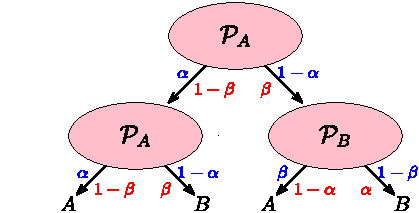
\includegraphics[scale = 1]{figures/composition_1.pdf}
\par\end{centering}
\caption{Standard composition of Coin flipping protocols. Subprotocols only have two outcomes depending on the coin flip. Labels indicate probabilities of outcomes for cheating Alice (blue) and cheating Bob (red)} 
\end{figure}
}
\begin{thm}
Let $X\in\{A,B\}$ and $\mathcal{X}\in\{\mathcal{I},\mathcal{Q}\}$.
Then $p_{X}^{*}(C^{LL}(\mathcal{P}))\approx0.8199\dots$ and $p_{X}^{*}(C^{LL}(\mathcal{X}))\approx0.836\dots$. 
\end{thm}


\subsection{Abort Phobic Compositions | $C^{L\perp},C^{\perp L}$}

\branchcolor{purple}{We now look at the case of abort phobic compositions, $C^{L\perp}$
and $C^{\perp L}$. We work through essentially the same example as
above and see what changes in this setting. Consider protocol $\mathcal{P}$
(see ...) and recall that as before 
\begin{align*}
p_{A}^{*}(\mathcal{P}_{A}) & =:\alpha\approx0.852\dots,\\
p_{B}^{*}(\mathcal{P}_{A}) & =:\beta\approx0.667\dots.
\end{align*}
In addition, we know from \Lemref{AliceSelfTests} that cheat vectors
for Bob, $(\alpha,\beta,\gamma)\in\mathbb{C}_{B}(\mathcal{P}_{A})$
admit a nice characterisation courtesy of the self testing step. Let
$\mathcal{P}':=C^{\perp L}(\mathcal{P},\mathcal{P})$, i.e. Alice
and Bob execute $\mathcal{P}_{A}$ and if the outcome is $A$, they
execute $\mathcal{P}_{A}$ while if the outcome is $B$, they execute
$\mathcal{P}_{B}$. Bob is assumed to be lenient so an honest Bob
never outputs abort, $\perp$. However, an honest Alice can output
abort, $\perp$ so we keep that output in the illustration, \Lemref{AliceSelfTests}.
Our goal is to find $p_{A}^{*}(\mathcal{P}')$ and $p_{B}^{*}(\mathcal{P}')$.
The former is the same as before because Bob is lenient: 
\[
p_{A}^{*}(\mathcal{P}')=\alpha\cdot\alpha+(1-\alpha)\cdot\beta.
\]
Clearly, $p_{B}^{*}(\mathcal{P}')\le\beta\alpha+(1-\beta)\beta$ but
this bound may not be tight because $(1-\beta)$ is the combined probability
of Alice aborting and Alice outputting $A$. However, we can use cheat
vectors to obtain 
\[
p_{B}^{*}(\mathcal{P}')=\max_{(v_{A},v_{B},v_{\perp})\in\mathbb{C}_{B}}v_{B}\alpha+v_{A}\beta
\]
which is an SDP one can solve numerically. Unlike the previous case,
the polarity of the resulting protocol, $\mathcal{P}'$, might have
flipped (compared to the polarity of $\mathcal{P}$). 

Repeating this procedure, one can consider $\mathcal{P}'':=C^{\perp L}(\mathcal{P},\mathcal{P}')$
and obtain $p_{A}^{*}(\mathcal{P}'')$ directly as illustrated above
and numerically solve for $p_{B}^{*}(\mathcal{P}'')$ using the cheat
vectors. Numerically, we found that ten-fifteen repetitions caused
the cheating probabilities to converge to approximately $0.81459$.
We saw that the abort probabilities associated with $\mathcal{P}$
were quite small and therefore one could hope that $\mathcal{Q}$
fares better. Proceed analogously for protocol and considering $\mathcal{Q}':=C^{L\perp}(\mathcal{Q},\mathcal{Q})$,
$\mathcal{Q}'':=C^{L\perp}(\mathcal{Q},\mathcal{Q}')$, etc., the
cheating probabilities converge to approximately $0.822655$. 

\begin{figure}
\begin{centering}
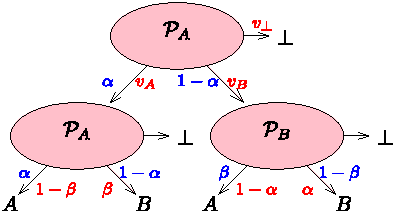
\includegraphics[scale=1]{figures/composition_2.pdf}
\par\end{centering}
\caption{Abort phobic compositing for Coin flipping protocols. Subprotocols have three possible outcomes including an abort symbol. Aborting in any subprotocol directly leads to aborting the whole protocol. Labels indicate probabilities of outcomes for cheating Alice (blue) and cheating Bob (red). In the security analysis of cheating Bob, we need to optimise over the cheat vectors  $(v_{A},v_{B},v_{\perp})\in\mathbb{C}_{B}$.
  \label{fig:Abort-Augmented-Composition}}
\end{figure}
}
\begin{thm}
Let $X\in\{A,B\}$. Then 
\[
p_{X}^{*}(C^{\perp L}(\mathcal{P}))\approx0.81459
\]
and 
\[
p_{X}^{*}(C^{L\perp}(\mathcal{Q}))\approx0.822655
\]
where the latter holds assuming Conjecture ?? is true. 
\end{thm}

\branchcolor{purple}{While by itself $\mathcal{Q}$ doesn't seem to help, one can suppress
the bias further, by noting that at the very last step, only the cheating
probabilities $p_{A}^{*}(\mathcal{Q})$ and $p_{B}^{*}(\mathcal{Q})$
played a role (i.e. the fact that the cheating vectors $\mathbb{C}_{A}$
for $\mathcal{Q}$ had an SDP characterisation was not used). Further,
we know that $p_{A}^{*}(\mathcal{P})=p_{A}^{*}(\mathcal{Q})$ but
$p_{B}^{*}(\mathcal{P})<p_{B}^{*}(\mathcal{Q})$, i.e. using $\mathcal{P}$
at the very last step will result in a strictly better protocol. }
\begin{thm}
Let $X\in\{A,B\}$, 
\begin{align*}
\mathcal{Z}^{1} & :=C^{L\perp}(\mathcal{Q},\mathcal{P}),\quad{\rm and}\\
\mathcal{Z}^{i+1} & :=C^{L\perp}(\mathcal{Q},\mathcal{Z}^{i})\quad i>1.
\end{align*}
Then 
\[
\lim_{i\to\infty}p_{X}^{*}(\mathcal{Z}^{i})\approx0.791044\dots
\]
assuming Conjecture ?? holds. 
\end{thm}


\section{Security Proof | Asymptotic limit}
\label{sec:securityAsymptotic}

In this section, we prove the security under the following assumption:
\begin{assumption}
\label{assu:asymptotic}In protocol $\mathcal{P}$ ($\mathcal{Q}$),
Alice (Bob) does not perform the box verification step and instead
it is assumed that her box is (his boxes are) taken from a trio of
boxes which win the GHZ game with certainty. 
\end{assumption}

\branchcolor{purple}{Later, we drop the assumption and use the box verification step (see
..) to estimate the probability of winning the GHZ game. When the
winning probability is exactly one, the states and measurements are
the same as the GHZ state and $\sigma_{x},\sigma_{y}$ measurements,
up to local isometries and this allows us to use semi definite programming. }
\begin{lem}
\label{lem:self-testAsymptotic}Let $a,b,c,x,y,z\in\{0,1\}$. Consider
a trio of quantum boxes, specified by projectors $\{M_{a|x}^{A},M_{b|y}^{B},M_{c|z}^{C}\}$
acting on finite dimensional Hilbert spaces $\mathcal{H}^{A},\mathcal{H}^{B}$
and $\mathcal{H}^{C}$, and $\left|\psi\right\rangle \in\mathcal{H}^{A}\otimes\mathcal{H}^{B}\otimes\mathcal{H}^{C}=:\mathcal{H}^{ABC}$.
If the trio pass the GHZ test with certainty, then there exists a
local isometry 
\[
\Phi=\Phi^{A}\otimes\Phi^{B}\otimes\Phi^{C}:\mathcal{H}^{ABC}\to\mathcal{H}^{ABC}\otimes\mathbb{C}^{2\times3}
\]
such that 
\begin{align*}
\Phi\left(\left|\psi\right\rangle \right) & =\left|\chi\right\rangle \otimes\left|{\rm junk}\right\rangle ,\\
\Phi\left(M_{d|t}^{D}\left|\psi\right\rangle \right) & =\Pi_{d|t}^{D}\left|{\rm GHZ}\right\rangle \otimes\left|{\rm junk}\right\rangle \quad\forall D\in\{A,B,C\},\text{ and }d,t\in\{0,1\}
\end{align*}
where $\left|{\rm GHZ}\right\rangle =\frac{\left|000\right\rangle +\left|111\right\rangle }{\sqrt{2}}\in\mathbb{C}^{2\times3}$,
$\left|{\rm junk}\right\rangle \in\mathcal{H}^{ABC}$ is some arbitrary
state and $\{\Pi_{a|x}^{A},\Pi_{b|y}^{B},\Pi_{c|z}^{C}\}$ are projectors
corresponding to $\sigma_{x}$ on the first, second and third qubit
of $\left|{\rm GHZ}\right\rangle $ respectively, for $x=0$ and corresponding
to $\sigma_{y}$ for $x=1$, as in \Claimref{Quantum-boxes-pass}.
\end{lem}

\branchcolor{purple}{INTERNAL; (TODO: remove): Isometries can only increase dimensions
(they must be injective; that is to ensure they preserve inner products
of vectors). Therefore the isometry can't get rid of the $\left|{\rm junk}\right\rangle $
part. }


\subsection{SDP when Alice self-tests\label{subsec:SDP-when-Alice}}

\branchcolor{blue}{\begin{proof}[Asymptotic proof of \Lemref{AliceSelfTests}]
We prove \Lemref{AliceSelfTests} under \Assuref{asymptotic}. We
begin by making two observations. 

First, note that in the protocol, if Alice applies an isometry on
her box \emph{after} she has inputted $x$, obtained the outcome $a$
(and has noted it somewhere), the security of the resulting protocol
is unchanged because the rest of the protocol only depends on $x$
and $a$, and Alice's isometry only amounts to relabelling of the
post measurement state. This freedom allows us to simplify the analysis.

Second, in the analysis, we cannot model Alice's random choice, say
for $x$, as a mixed state because Bob can always hold a purification
and thus know $x$. Therefore, we model the randomness using pure
states and measure them in the end.

Notation: Other than $PQR$, all other registers store qubits.

We proceed step by step. 
\begin{enumerate}
\item We can model (justified below) Alice's act of inputting a random $x$
and obtaining an outcome $a$ from her box through the state 
\begin{equation}
\left| \Psi_{0} \right\rangle :=\frac{1}{2}\sum_{x,a\in\{0,1\}}\left|xa\right\rangle _{XA}\left|\Phi(x,a)\right\rangle _{IJ}
\end{equation}
where $X$ represents the random input and $A$ the output. Here,
$\left|\Phi(x,a)\right\rangle _{IJ}$ are Bell states (see \Eqref{bellStates})
and the registers $IJ$ are held by Bob. Alice's act of choosing $r$
at random, computing $s=a\oplus x.r$ is modelled as 
\begin{equation}
\left|\Psi_{1}\right\rangle :=\frac{1}{2\sqrt{2}}\sum_{x,a,r\in\{0,1\}}\left|xa\right\rangle _{XA}\left|\Phi(x,a)\right\rangle _{IJ}\left|r\right\rangle _{R}\left|a\oplus x.r\right\rangle _{S}.\label{eq:Alice_Psi1}
\end{equation}
Finally, Alice's act of sending $s$ is modelled as Alice starting
with the state
\[
\tr_{IJS}\left[\left|\Psi_{1}\right\rangle \left\langle \Psi_{1}\right|\right]\in XAR.
\]
\Tnote{Can we call this state $\rho_1$ ?}


\branchcolor{blue}{\textbf{Justification for starting with $\left|\Psi_{0}\right\rangle $.}\\
To see why we start with the state $\left|\Psi_{0}\right\rangle $,
model Alice's choice of $x$ as $\left|+\right\rangle _{X}$, suppose
her measurement result is stored in $\left|0\right\rangle _{A}$,
the state of the boxes before measurement is $\left|\psi\right\rangle _{PQR}$
and Alice holds $P$, i.e. 
\[
\left|\Psi_{0}'\right\rangle :=\left|+\right\rangle _{X}\left|0\right\rangle _{A}\left|\psi\right\rangle _{PQR}.
\]
Let $\{M_{a|x}^{P}\}$ be the measurement operators corresponding
to Alice's box. The measurement process is unitarily modelled as 
\[
\left|\Psi_{1}'\right\rangle :=U_{{\rm measure}}\left|\Psi_{0}'\right\rangle =\frac{1}{\sqrt{2}}\sum_{x,a\in\{0,1\}}\left|x\right\rangle _{X}\left|a\right\rangle _{A}M_{a|x}^{P}\left|\psi\right\rangle _{PQR}
\]
where
\[
U_{{\rm measure}}=\sum_{x\in\{0,1\}}\left|x\right\rangle \left\langle x\right|_{X}\otimes\left[\mathbb{I}_{A}\otimes M_{0|x}^{P}+X_{X}\otimes M_{1|x}^{P}\right]\otimes\mathbb{I}_{QR}.
\]
Now we harness the freedom of applying an isometry to the post measured
state (as observed above). We choose the local isometry in \Lemref{self-testAsymptotic}.
Without loss of generality, we can assume that Bob had already applied
his part of the isometry before sending the boxes (because he can
always reverse it when it is his turn). We thus have, 
\begin{align*}
\left|\Psi_{2}'\right\rangle :=\Phi_{PQR}\left|\Psi_{1}'\right\rangle  & =\frac{1}{\sqrt{2}}\sum_{x,a\in\{0,1\}}\left|x\right\rangle _{X}\left|a\right\rangle _{A}\Pi_{x|a}^{H}\left|{\rm GHZ}\right\rangle _{HIJ}\otimes\left|{\rm junk}\right\rangle _{PQR}\\
 & =\frac{1}{2}\sum_{x,a\in\{0,1\}}\left|x\right\rangle _{X}\left|a\right\rangle _{A}U^{H}(x,a)\left|0\right\rangle _{H}\left|\Phi(x,a)\right\rangle _{IJ}\otimes\left|{\rm junk}\right\rangle _{PQR}
\end{align*}
where 
\begin{equation}
\left|\Phi(x,a)\right\rangle _{IJ}=\frac{\left|00\right\rangle +(-1)^{a}(i)^{x}\left|11\right\rangle }{\sqrt{2}}\label{eq:bellStates}
\end{equation}
 and $U^{H}(x,a)\left|0\right\rangle _{H}$ is $\frac{\left|0\right\rangle +(-1)^{a}(i)^{x}\left|1\right\rangle }{\sqrt{2}}$.
Since the state of register $H$ is completely determined by registers
$X$ and $A$, we can drop it from the analysis without loss of generality.
Finally, since $\left|{\rm junk}\right\rangle _{PQR}$ is completely
tensored out, we can drop it too without affecting the security. Formally,
we can assume that Alice gives Bob the register $P$ at this point.
}
\item Bob sending $g$ is modelled by introducing $\rho_{2}\in XARG$ satisfying
$\tr_{IJS}\left[\left|\Psi_{1}\right\rangle \left\langle \Psi_{1}\right|\right]=\tr_{G}(\rho_{2})$. 
\item At this point, either $x\oplus g$ is zero, in which case Alice's
output is fixed or $x\oplus g$ is one, and in that case Bob will
already know $x$ because he knows $g$ (he sent it) and Alice will
proceed to testing Bob. Formally, therefore, we needn't do anything
at this step.
\item Assuming $x\oplus g=1$, Alice sends $y,z$ to Bob such that $x\oplus y\oplus z=1$.
However, since Bob already knows $x$, he can deduce $z$ from $y$.
We thus only need to model Alice sending $y$ and Bob responding with
$d=b\oplus c$ (because Alice will only use $b\oplus c$ to test the
GHZ game, so it suffices for Bob to send $d$). This amounts to introducing
$\rho_{3}\in XARGYD$ satisfying $\rho_{2}\otimes\frac{\mathbb{I}_{Y}}{2}=\tr_{D}(\rho_{3})$. 
\item Since we postponed the measurements to the end, we add this last step.
Alice now measures $\rho_{3}$ to determine $x\oplus g$ and if it
is one, whether the GHZ test passed. Let 
\begin{align}
\Pi_{i} & :=\sum_{x,y\in\{0,1\}:x\oplus g=i}\left|xg\right\rangle \left\langle xg\right|_{XG}\otimes\mathbb{I}_{ARYD},\nonumber \\
\Pi^{{\rm GHZ}} & :=\sum_{\substack{x,y\in\{0,1\},\\
a,d\in\{0,1\}:a\oplus d\oplus1=xy\cdot(1\oplus x\oplus y)
}
}\left|xyad\right\rangle \left\langle xyad\right|_{XYAD}\otimes\mathbb{I}_{RG}.\label{eq:AliceProjs}
\end{align}
Then, we can write the cheat vector for Alice, i.e. the tuple of probabilities
that Alice outputs 0, 1 and abort (see \Defref{CheatVectors}), as
\[
(\alpha,\beta,\gamma)=(\tr(\Pi_{0}\rho_{3}),\tr(\Pi_{1}\Pi^{{\rm GHZ}}\rho_{3}),\tr(\Pi_{1}\bar{\Pi}^{{\rm GHZ}}\rho_{3}))
\]
 where $\bar{\Pi}:=\mathbb{I}-\Pi$.
\end{enumerate}
To summarise, the final SDP is as follows: let $\left|\Psi_{1}\right\rangle \in XAIJRS$
be as given in \Eqref{Alice_Psi1}, $\rho_{2}\in XARG$ and $\rho_{3}\in XARGYD$
\[
\max\quad\tr([c_{0}\Pi_{0}+\Pi_{1}(c_{1}\Pi^{{\rm GHZ}}+c_{\perp}\bar{\Pi}^{{\rm GHZ}})]\rho_{3})
\]
subject to 
\begin{align*}
\tr_{IJS}\left[\left|\Psi_{1}\right\rangle \left\langle \Psi_{1}\right|\right] & =\tr_{G}(\rho_{2})\\
\rho_{2}\otimes\frac{\mathbb{I}_{Y}}{2} & =\tr_{D}(\rho_{3})
\end{align*}
where the projectors are defined in \Eqref{AliceProjs}.
\end{proof}
}


\subsection{SDP when Bob self-tests\label{subsec:SDP-when-Bob}}

\branchcolor{blue}{\begin{proof}[Proof of \Lemref{Bob-self-tests}]
Denote by $\mathcal{I}$ the protocol corresponding to \Algref{SCForiginal}. 

It is evident that $p_{B}^{*}(\mathcal{Q})\le p_{B}^{*}(\mathcal{I})$
because compared to $\mathcal{I}$, in $\mathcal{Q}$ Alice performs
an extra test. However, it is not hard to see that the inequality
is saturated, i.e. $p_{B}^{*}(\mathcal{Q})=p_{B}^{*}(\mathcal{I})$.
Consider ... (TODO: recall/re-construct the cheating strategy for
Bob that lets him win with the same $3/4$ probability). 

From \Lemref{SCFstandard}, it is also clear that $p_{A}^{*}(\mathcal{Q})=p_{A}^{*}(\mathcal{I})$
because the only difference between Bob's actions in $\mathcal{Q}$
and $\mathcal{I}$ is that Bob self-tests to ensure his boxes are
indeed GHZ. However, the optimal cheating strategy for $\mathcal{I}$
can be implemented using GHZ boxes. 

This establishes the first part of the lemma. For the second part,
i.e. establishing that optimising $c_{0}\alpha+c_{1}\beta+c_{\perp}\gamma$
over $(\alpha,\beta,\gamma)\in\mathbb{C}_{A}$ is an SDP, we proceed
as follows. Suppose \Assuref{asymptotic} holds. Then we can assume
that Bob starts with the state 
\begin{equation}
\rho_{0}:=\tr_{H}(\left|{\rm GHZ}\right\rangle \left\langle {\rm GHZ}\right|_{HIJ})\label{eq:Bob_initState}
\end{equation}
 and the effect of measuring the two boxes can be represented by the
application of projectors of pauli operators $X$ and $Z$.

The justification is similar to that given in the former proof. Suppose
Bob holds registers $QR$ of $\left|\psi\right\rangle _{PQR}$ which
is the combined state of the three boxes. Suppose his measurement
operators are $\{M_{b|y}^{Q},M_{c|z}^{R}\}$. Then using the isometry
in \Lemref{self-testAsymptotic}, Bob can relabel his state (and without
loss of generality, we can suppose Alice also relabels according to
the aforementioned isometry) to get $\Phi_{PQR}\left|\psi\right\rangle _{PQR}=\left|{\rm GHZ}\right\rangle _{HIJ}\otimes\left|{\rm junk}\right\rangle _{PQR}$.
Further, since $\Phi_{PQR}(M_{b|y}^{Q}\otimes M_{c|z}^{R}\left|\psi\right\rangle _{PQR})=\Pi_{b|y}^{I}\Pi_{c|z}^{J}\left|{\rm GHZ}\right\rangle _{HIJ}\otimes\left|{\rm junk}\right\rangle _{PQR}$
Bob's act of measurement, in the new labelling, corresponds to simply
measuring the GHZ state in the appropriate Pauli basis. (TODO: in
the approximate case, the initial state will be close to the one mentioned
and the post-measured state will similarly only be close to the one
post projectors; There should be some way of showing that this can
be absorbed into the initial state).
\Tnote{There is still a TODO here}
\begin{enumerate}
\item Bob receiving $s$ from Alice is modelled by introducing $\rho_{1}\in SIJ$
satisfying $\tr_{S}(\rho_{1})=\rho_{0}$. 
\item Bob sending $g\in_{R}\{0,1\}$ can be seen as appending a mixed state:
$\rho_{1}\otimes\frac{1}{2}\mathbb{I}_{G}$.
\item Alice sending $x$ (and $a$) can be modelled as introducing $\rho_{2}\in AXSIJG$
satisfying $\tr_{A}(\rho_{2})=\rho_{1}\otimes\frac{\mathbb{I}_{G}}{2}$.
\item To model the GHZ test, introduce a register $Y$ in the state $\frac{\left|0\right\rangle _{Y}+\left|1\right\rangle _{Y}}{\sqrt{2}}$.
Recall that to perform the GHZ test, we need $x\oplus y\oplus z=1$
i.e. $z=1\oplus y\oplus x$. Further introduce registers $B$ and
$C$ to hold the measurement results, define 
\begin{equation}
U:=\sum_{y,x\in\{0,1\}}\left|y\right\rangle \left\langle y\right|_{Y}\left|x\right\rangle \left\langle x\right|_{X}\otimes(\mathbb{I}_{B}\otimes\Pi_{0|y}^{I}+X_{B}\otimes\Pi_{1|y}^{I})\otimes(\mathbb{I}_{C}\otimes\Pi_{0|(1\oplus y\oplus x)}^{J}+X_{C}\otimes\Pi_{1|(1\oplus y\oplus x)}^{J})\otimes\mathbb{I}_{ASG}.\label{eq:Bob-u}
\end{equation}
By construction, $\rho_{3}:=U\left(\left|+\right\rangle \left\langle +\right|_{Y}\otimes\left|00\right\rangle \left\langle 00\right|_{BC}\otimes\rho_{2}\right)U^{\dagger}\in YBCAXSIJG$
models the measurement process. (TODO: this equality would become
approximately true...but perhaps the noise can be absorbed in $\rho_{0}$
with some argument)
\item Since we postponed the measurements to the end, we add this step.
Define 
\[
\Pi_{i}:=\sum_{x,g\in\{0,1\}:x\oplus g=i}\left|xg\right\rangle \left\langle xg\right|_{XG}\otimes\mathbb{I}_{YABSIJ}
\]
to determine who won. Define 
\[
\Pi^{{\rm sTest}}:=\sum_{s,a,x\in\{0,1\}:s=a\lor s=a\oplus x}\left|sax\right\rangle \left\langle sax\right|_{SAX}\otimes\mathbb{I}_{GYBCIJ}
\]
 to model the first test, i.e. $s$ should either be $a$ or $a\oplus x$.
Define 
\[
\Pi^{{\rm GHZ}}:=\sum_{\substack{x,y\in\{0,1\},\\
a,b,c\in\{0,1\}:a\oplus b\oplus c\oplus1=xy\cdot(1\oplus x\oplus y)
}
}\left|xyabc\right\rangle \left\langle xyabc\right|_{XYABC}\otimes\mathbb{I}_{GSIJ}
\]
to model the GHZ test. Let 
\begin{equation}
\Pi^{{\rm Test}}:=\Pi^{{\rm GHZ}}\Pi^{{\rm sTest}},\quad\bar{\Pi}^{{\rm Test}}:=\mathbb{I}-\Pi^{{\rm Test}}.\label{eq:BobProjs}
\end{equation}
One can then write the cheat vector for Bob, i.e. the tuple of probabilities
that Bob outputs $0,1$ and abort (see \Defref{CheatVectors}), as
\[
(\alpha,\beta,\gamma)=(\tr(\Pi_{0}\Pi^{{\rm Test}}\rho_{3}),\tr(\Pi_{1}\rho_{3}),\tr(\Pi_{0}\bar{\Pi}^{{\rm Test}}\rho_{3})).
\]
\end{enumerate}

\Tnote{NB: Still old notation for the cheat vectors}
To summarise, the final SDP is as follows: let $\rho_{0}\in IJ$ be
as defined in \Eqref{Bob_initState}, $\rho_{1}\in SIJ$ and $\rho_{2}\in AXSIJG$.
Then, 
\[
\max\quad\tr\left([\Pi_{0}(c_{0}\Pi^{{\rm Test}}+c_{\perp}\bar{\Pi}^{{\rm Test}})+c_{1}\Pi_{1}]U\left(\left|+00\right\rangle \left\langle +00\right|_{YBC}\otimes\rho_{2}\right)U^{\dagger}\right)
\]
subject to 
\begin{align*}
\tr_{S}(\rho_{1}) & =\rho_{0}\\
\tr_{A}(\rho_{2}) & =\frac{1}{2}\rho_{1}\otimes\mathbb{I}_{G}
\end{align*}
where $U$ is as defined in \Eqref{Bob-u} and the projectors as in
\Eqref{BobProjs}.


\end{proof}
}

\section{Security Proof | Finite $n$}
\label{sec:SecurityFiniteN}
TODO: Write the following properly

In this section, we drop Assumption ??, and estimate the GHZ winning probability from Algorithm ??. We then use the robust variant of the self-testing result to conclude that the SDP of interest must be close to the SDP we considered (with some larger space tensored to it). Finally, we show the continuity of these SDPs and thereby conclude that we converge to the asymptotic result as $n$ is increased.

We show this for the case where Alice self-tests. We expect an analogous result to hold when Bob self-tests.


\subsection{Estimation of GHZ winning probability}
\label{subsec:EstimateGHZ}
We assume that the $3n$ boxes are described by some joint quantum state and local measurement operators. After playing the GHZ game with $3(n-1)$ of them, and verifying that they all pass, we want to make a statement about the remaining box, whose state $\tilde \rho$ is conditioned on the passing of all the other test. 

% \begin{algorithm}[H]
% \label{alg:self-test}
% \caption{Estimation of the GHZ value}
% \begin{algorithmic}[1]
%     \STATEx 
% 	\STATE Pick a box $J \in [ n ]$ uniformly at random.
% 	\STATE For $i \in [n]\backslash J$, play the GHZ game with box $i$, denote outcome of game as $X_i\in \{0,1\}$ 
% 	\STATE If 
% 	\begin{IEEEeqnarray}{r'L}
% 	     \Omega:& X_i = 1 \text{, for all } i\in [n] \backslash J
% 	\end{IEEEeqnarray}
% 	\STATE Then conclude that the remaining box satisfies
% 	\begin{IEEEeqnarray}{r'L}
% 	     T:& E[X_J|J,\Omega] \geq 1 - \delta 
% 	\end{IEEEeqnarray}
% \end{algorithmic}
% \end{algorithm}

\begin{lyxalgorithm}
	\label{alg:self-test} Estimation of the GHZ value.
	% \caption{Estimation of the GHZ value}
	% \begin{algorithmic}[1]
	%     \STATEx 
	\begin{enumerate}
		\item Pick a box $J \in [ n ]$ uniformly at random.
		\item For $i \in [n]\backslash J$, play the GHZ game with box $i$, denote outcome of game as $X_i\in \{0,1\}$ 
		\item If 
		\begin{IEEEeqnarray}{r'L}
		     \Omega:& X_i = 1 \text{, for all } i\in [n] \backslash J
		\end{IEEEeqnarray}
		\item Then conclude that the remaining box satisfies
		\begin{IEEEeqnarray}{r'L}
		     T:& E[X_J|J,\Omega] \geq 1 - \delta 
		\end{IEEEeqnarray}
	\end{enumerate}
	% \end{algorithmic}
\end{lyxalgorithm}
	
The expectation value of $E[X_J|J,\Omega]$ accurately describes the expected GHZ value associated to the state of the remaining boxes $J$, conditioned on having measuring some outcome sequence in the other boxes which passes all the GHZ tests. Note that the conditioning in $J$ is important because otherwise we would get a bound on the GHZ averaged over all boxes, but we are only interested in the remaining box.

\begin{prop}[Security of \Algref{self-test}]
	\label{prop:security}
	For any implementation of the boxes and choice of $\delta>0$ the joint probability that that the test $\Omega$ passes and that the conclusion $T$ is false is small $\Pr[ \Omega \cap \bar T] \leq \frac{1}{1-\delta + n\delta} \leq \frac{1}{n\delta}$, where the first upper-bound is tight.
\end{prop}

This is the correct form of the security statement. It is important to bound the joint distribution of $\Omega$ and $\overline T$, and not $\Pr[\overline T|\Omega]$, conditioning on passing the test $\Omega$. Indeed in the latter case, it would not be possible to conclude anything of value about the remaining box $J$, as there could be some implementation of the boxes which has a very low expectation value of GHZ, but which passes the test with small but non-zero probability. The present security definition has a nice interpretation in the composable security framework of [ref]. Consider an hypothetical ideal protocol, which after having chosen $J$, only passes when $T$ is true. In that case, $\Pr[\Omega\cap \overline T] = 0$. Then the actual protocol is equivalent the ideal one, except that if fails with probability $\epsilon = \frac{1}{1-\delta + m\delta}$, and so it is $\epsilon$-close to the ideal algorithm. 


\begin{proof}
	For a given implementation of the boxes, let $p(x_1,\cdots x_n)$ denote the joint probability distribution of passing the GHZ games. Let $S = \{j|\ E[X_j|J=j, \Omega] < 1-\delta\} \subset [n]$ be the set of boxes that have an expectation value for GHZ (conditioned on passing in the other boxes) below our target threshold and let $m = |S|$ be the number of such boxes. The value of $m$ is unknown, so we will need to maximise over it in the end.
	
	Let $\alpha = \Pr(\{X_i\}_i = 1)$ and $\beta_i = \Pr(\{X_i\}_{i\neq j} = 1 \cap X_j = 0)$ be respectively the probabilities of the events where all the tests pass, or they all pass except for the $j$th test. This allows us to rewrite $E[X_j|J=j,\Omega] = \Pr(\{X_i\}_i=1)/\Pr(\{X_i\}_{i\neq j} = 1) = \alpha/(\alpha + \beta_j)$, and so, by definition of $S$, we have $ \alpha/(\alpha + \beta_j)<(1-\delta)$, for $j\in S$, which is equivalent to $\beta_j > \frac{\delta}{1-\delta} \alpha$. 
	
	The aim of the proof is to bound the probability $\Pr[\Omega \cap \overline T]$. If we condition and summed over the different values of $J$, we can rewrite it as
    \begin{IEEEeqnarray}{rL}
         \Pr(\Omega \cap \overline T) = \sum_j \frac{1}{n} \Pr(\Omega \cap \overline{T}| J = j) = \sum_{j\in S} \frac{1}{n} \Pr(\{X_i\}_{i\neq j} = 1) = \frac{1}{n} \sum_{j\in S} (\alpha + \beta_i)\,,
    \end{IEEEeqnarray}
    where we have kept the round $j\in S$ ones, conditioned on which $T$ is false. 
    We are thus left with the optimisation problem 
	\begin{IEEEeqnarray}{L'L}
		\max_{\alpha\geq 0,(\beta_i)_i\geq 0} 	
		    &\frac{1}{n}\left( \sum_{j\in S} \alpha + \beta_j\right)\\
		\mathrm{subject\ to}					
		    &\alpha + \sum_{j\in S} \beta_j \leq 1\\
			& \beta_j \geq \frac{\delta}{1-\delta} \alpha \text{, for }j\in S		
	\end{IEEEeqnarray}	    
	This is a linear problem. Simplifying it by defining $\Sigma = \sum_{j\in S} \beta_j$, gives
	\begin{IEEEeqnarray}{L'L}
		\max_{\alpha\geq0,\Sigma\geq0} 	&\frac{1}{n}( m\alpha + \Sigma)\\
		\mathrm{subject\ to}					
		    &\alpha + \Sigma \leq 1\\
			& \Sigma \geq m\frac{\delta}{1-\delta} \alpha			
	\end{IEEEeqnarray}
	It is easily shown that the maximum is attained for $(\alpha,\Sigma) = \left(\frac{1-\delta}{1-\delta + m\delta}, \frac{m \delta}{1-\delta + m\delta}\right)$ which gives the upper-bound
	\begin{IEEEeqnarray}{rL}
		\Pr[\Omega\cap \overline T] \leq \frac{1}{n} \max_m \frac{m}{1-\delta + m\delta} = \frac{1}{1-\delta + n\delta}
	\end{IEEEeqnarray}
	We note that the upper-bound is an increasing function of $m$ and so the maximum is attained for $m=n$. This yield the desired upper-bound. From the converse statement, we note that from the present proof we can construct a probability distribution $p(x_1,\cdots x_n)$, which saturates all inequalities, and so the upper-bound $\frac{1}{1-\delta + n\delta}$ is tight.
\end{proof}


\subsection{Robust self-testing}
\begin{lem}
Let $a,b,c,x,y,z\in\{0,1\}$. Consider a trio of quantum boxes, specified
by projectors $\{M_{a|x}^{A},M_{b|y}^{B},M_{c|z}^{C}\}$ acting on
finite dimensional Hilbert spaces $\mathcal{H}^{A},\mathcal{H}^{B}$
and $\mathcal{H}^{C}$, and $\left|\psi\right\rangle \in\mathcal{H}^{A}\otimes\mathcal{H}^{B}\otimes\mathcal{H}^{C}=:\mathcal{H}^{ABC}$.
If the trio pass the GHZ test with probability $1-\epsilon$ (for
$1>\epsilon>0$), then there exists a local isometry, 
\[
\Phi=\Phi^{A}\otimes\Phi^{B}\otimes\Phi^{C}:\mathcal{H}^{ABC}\to\mathcal{H}^{ABC}\otimes\mathbb{C}^{2\times3}
\]
and a decreasing function of $\epsilon$, $f(\epsilon)$ such that
\begin{align}
    \label{eq:continuity_GHZ}
\left\Vert \Phi\left(\left|\psi\right\rangle \right)-\left|\chi\right\rangle \otimes\left|{\rm junk}\right\rangle \right\Vert  & \le f(\epsilon),\\
\left\Vert \Phi\left(M_{d|t}^{D}\left|\psi\right\rangle \right)-\Pi_{d|t}^{D}\left|{\rm GHZ}\right\rangle \otimes\left|{\rm junk}\right\rangle \right\Vert  & \le f(\epsilon)\quad\forall D\in\{A,B,C\},\text{ and }d,t\in\{0,1\}
\end{align}
where $\left|{\rm GHZ}\right\rangle =\frac{\left|000\right\rangle +\left|111\right\rangle }{\sqrt{2}}\in\mathbb{C}^{2\times3}$,
$\left|{\rm junk}\right\rangle \in\mathcal{H}^{ABC}$ is some arbitrary
state and $\{\Pi_{a|x}^{A},\Pi_{b|y}^{B},\Pi_{c|z}^{C}\}$ are projectors
corresponding to $\sigma_{x}$ on the first, second and third qubit
of $\left|{\rm GHZ}\right\rangle $ respectively, for $x=0$ and corresponding
to $\sigma_{y}$ for $x=1$, as in \Claimref{Quantum-boxes-pass}.
\end{lem}
\begin{proof}
    A proofs of robust self-testing for GHZ can be found in \cite{MillerShi} and \cite{McKague}.
\end{proof}

\subsection{SDP-valued functions and their continuity}
\label{subsec:SDPcontinuity}
A semidefinite program (SDP) is an optimization problem of the form 
\begin{align} 
f(A,B) = \text{maximize:} \quad & \ip{A}{X} \nonumber \\ 
\text{subject to:} \quad 
& \Phi(X) = B \label{SDP} \\ 
& X \geq 0. \nonumber
\end{align}  
We call $f(A,B)$ the value of the semidefinite program which is the supremum of $\ip{A}{X}$ over all $X$ that are feasible ($X \succeq 0$ and $\Phi(X) = B$). 
In this work we wish to view how the value of an SDP changes as you change $A$ and/or $B$. 
%To this end, we define the concept of a support function. 
Ultimately, we wish to know if the value of an SDP is continuous as a function of $A$ and $B$. 
To this end, let us consider the function 
\begin{align} 
h(A) = \text{maximize:} \quad & \ip{A}{X} \\ 
\text{subject to:} \quad 
& X \in C  
\end{align}   
where $C$ is a nonempty, convex set. 
This is a generalization of an SDP which is  convenient for the upcoming analysis.  
Notice that when $C$ is unbounded, it may be the case that $f$ takes the value $+ \infty$. 
Since we cannot count that high, we use the following definition. 

\begin{defn} 
We define the \emph{support} of the function $h$, denoted as $\supp(h)$, as 
\begin{equation} 
\supp(h) := \{ A : h(A) \textup{ is finite} \}.  
\end{equation} 
\end{defn} 

We now show some elementary properties of this function. 

\begin{lem} 
The support of $h$ is convex and $h$ is a convex function on its support. 
\end{lem} 

\begin{proof} 
%Since $C$ is convex, we have that $\lambda_1 A_1 + \lambda_2 A_2 \in C$ for all $A_1, A_2 \in C$ and $\lambda_1, \lambda_2 \geq 0$ satisfying $\lambda_1 + \lambda_2 = 1$. 
For $A_1, A_2 \in \supp(h)$ and $\lambda_1, \lambda_2 \geq 0$ satisfying $\lambda_1 + \lambda_2 = 1$, we have  
\begin{align}
h(\lambda_1 A_1 + \lambda_2 A_2) 
& \leq h(\lambda_1 A_1) + h(\lambda_2 A_2) \\ 
& = \lambda_1 h(A_1) + \lambda_2 h(A_2) \\ 
& < + \infty  
\end{align} 
where the last inequality follows from $A_1, A_2 \in \supp(h)$.  
Thus, $\lambda_1 A_1 + \lambda_2 A_2 \in \supp(h)$, proving $\supp(h)$ is a convex set, and $h$ is convex from the above inequalities. 
\end{proof} 

The following corollary follows from the fact that $h$ is convex. 

\begin{cor} \label{contint}
$h$ is continuous on the interior of its support. 
\end{cor} 

Another well-known corollary is that $h$ is 
continuous everywhere if $C$ is compact. 
This follows from the above corollary since the support is the entire space. 

\begin{cor} \label{contint}
If $C$ is compact, $h$ is continuous everywhere. 
\end{cor} 

\subsubsection{SDP approximation and finite statistics} 

\Jnote{Continue here.} 








\Jnote{references are incomplete. SCA+11 is missing first names. ARV missing year and journal and year. ARW is missing everything. Kit03 should probably have a link to the website. STOC references inconsistent. TQC refs inconsistent. Are ARW and ARW 19 the same?}


\clearpage
\bibliographystyle{amsalpha}
\bibliography{DI_WCF_ideas}

\end{document}
